
\chapter{Identification Under Domiciliary Conditions}
\label{sec:ExperimentalIntervalIdentification}

Exploring the feasibility of full patient characterization is the main objective of this thesis, and the results of the \textit{in silico} and in-patient in-clinic experimental identification were encouraging. However, many of the premises of the previous chapters are not realistic in the consideration of an ambulatory patient identification for the artificial pancreas. For practical purposes, a home-made patient identification must be performed over the information that a patient obtains in daily routine. This requires the use of CGM measurements for the glucose estimation signal, and either pump or periodic injections, as well as meal estimation.

The Identification methodology and the diabetic patient data for this chapter has already been presented in previous chapters. CMAES optimization algorithm was used for the minimization of the hybrid cost index explained in the study in Chapter \ref{sec:PilotExperimentalIdentification}. The hybrid index is not different from that explained previously, and the only difference remains in the vector of parameters to be optimized.

\section{Optimization settings and parameters}
\label{sec:OptimizationSettingsAndParameters}

In this chapter identification is performed realistically on a full physiologic model of a diabetic patient. The model used for the identification included, unlike the previous chapter, a system for the subcutaneous insulin absorption. This subsystem is known to suffer from enormous variability, and as such it is well suited for characterization from interval models. The insulin absorption model used was the one included in the Cambridge simulator, in order to keep coherence with the rest of the models used. The parameter $k_a$ defined in Chapter \ref{sec:WillinskaEtAl} is referred here as $t_{maxI}$ in order to keep the same notation for both the insulin and glucose absorption models.

In the case of insulin pump usage, which is the case of the dataset used, there is also the possibility of pump-induced errors (in terms of deviations of the actual delivered insulin dose from the programmed dose, as can be caused by total or partial occlusions of the infusion set), probably caused by total or partial occlusions. This type of errors is very similar to the estimation errors present in the amount of CHO of a meal. A very similar approach to that of the multiplicative aggregated parameter $\alpha$ in the gastrointestinal system was used here to gather all uncertainties in the insulin model input into one single multiplicative parameter, defined $\beta$. This parameter was treated as an interval parameter and tested for identification capabilities in the following.

The other parameter influencing the insulin absorption is the insulin elimination rate from plasma $k_e$. This parameter was identified considering variability. Exactly in the same way as with the gastrointestinal model (in the $t_{maxG}$ parameter), the flux constant $t_{maxI}$ was identified on every patient, but due to the already mentioned interval model implementation limitations, no uncertainty was considered for it, so it was considered a constant value on each patient for the whole duration of the experiment. In practice, little difference exists when considering the uncertainty in the parameter $\beta$ or in the $t_{maxI}$ parameter when fitting experimental data, similarly to what happened when comparing $t_{maxG}$ and $\alpha$ in the gastrointestinal model. Very simple simulations of uncertainty are displayed in Figure \ref{fig:tmaxI_ke_ins} for both the $\beta$ parameter and $t_{maxI}$.

\begin{figure}[hbtp]
\centering
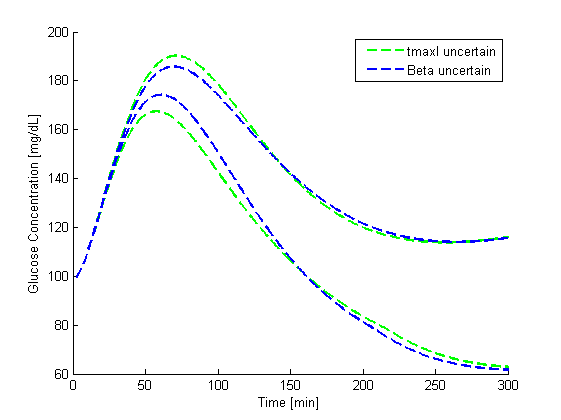
\epsfig{file=Figures/tmaxI_ke_ins_laguna.png, width=0.8\textwidth}\caption{Simulation of a postprandial period considering a 15\% uncertainty in the parameter $t_{maxI}$ (in green) or in the aggregated parameter $\beta$ (blue).}
\label{fig:tmaxI_ke_ins}
\end{figure}

Both parameters have virtually no influence in the envelope width of the glucose profile in the 45 minutes following the meal intake. Beyond that time $t_{maxI}$ may present larger uncertainty, but its influence is negligible, even being the glucose envelopes very similar in the late postprandial period (two hours after ingestion). Even though the simulation shown in the gastrointestinal model showed better similarities between the parameters under comparison, the simulations for the model of subcutaneous insulin infusion are still considered to be very similar from a practical point of view. Again, it is worth mentioning that these models will be used for data fitting, so the envelopes shown in Figure \ref{fig:tmaxI_ke_ins} are but a qualitative representation of the uncertainty related to each parameter throughout the postprandial period.

Finally, the complete set of parameters for identification is:

\begin{equation}\label{eq:parametervectorCGM}
%\begin{split}
\theta=[ \underline{S_{iT}}, \overline{S_{iT}}, \underline{S_{iD}}, \overline{S_{iD}}, \underline{S_{iE}}, \overline{S_{iE}}, \underline{k_{12}}, \overline{k_{12}}, \underline{k_e}, \overline{k_e}, \underline{\alpha}, \overline{\alpha}, \underline{\beta}, \overline{\beta}, t_{maxI}, t_{maxG} ]
%\end{split}
\end{equation}

The parameter set proposed is equivalent to that used in the \textit{in silico.} identifications.

The selection of the value for $\gamma$ is one of the most important discussions in the completion of any identification with the proposed hybrid index. The selection of an appropriate $\gamma$ is dependent on the type of the data being fitted, and of the error expected in the measurements in particular. The larger the error on the measurements is, the less importance is assigned to the fit part of the composite index. This approach is the opposite to the error-bound estimation explained in Chapter \ref{sec:ErrorBoundedEstimation}, where the parameter set searched was of those parameters that are consistent with the data and its error. That approach leads to larger parameter sets as the uncertainty grows in the measurement. In the approach used here works exactly on the opposite way, ensuring a minimum set of parameters that are consistent with the \emph{physiology} of the patient and the uncertainty in the patient, not on the measurements. Excessive width in the glucose envelope must be avoided, so the physiologic set of interval parameters must reduce its width for CGM experiments.

In the last chapter, a $\gamma$ value of 100 was considered appropriate for the data being fitted. In the case at stake now, the data available is less similar to the mathematical model output because physiologic approximations are introduced in the subcutaneous insulin model. Therefore, less accurate predictions are expected from the model used and fitting error may be desired to be fit more loosely to the broader set of data that CGM monitoring is (in comparison with glucose reference. In order to account for this, two different $\gamma$ values are tested for every combination of parameters considered in the identifications: $\gamma = 100$ and $\gamma = 50$. Having $\gamma = 100$ allows for comparison with previous results, because the error weighting is the same as in Chapter \ref{sec:PilotExperimentalIdentification}. In the case that $\gamma = 50$, reduces the influence of the fitting error for accounting with the exposed model mismatches.

For the selection of identification parameters, several identifications were performed on reference glucose for different parameter vectors. A total of eight different parameter sets were considered. The scenarios are detailed in Table \ref{tab:YSISCinsscenarios}. Note that the complete set of parameters being identified is detailed in equation \eqref{eq:parametervectorCGM}, and Table \ref{tab:YSISCinsscenarios} only shows the three interval parameters that were used in the permutations for the construction of the scenarios.

\begin{table}[hbtp]
	\centering
	\begin{tabular}{| c | c | c | c |}
	\hline
	\textbf{Scenario} & $\alpha$ & $\beta$ & $k_e$ \\
	\hline
	A & \cmark & \cmark & \cmark \\
  B & \cmark & \cmark & \xmark \\
	C & \cmark & \xmark & \cmark \\
	D & \cmark & \xmark & \xmark \\
	E & \xmark & \cmark & \cmark \\
	F & \xmark & \cmark & \xmark \\
	G & \xmark & \xmark & \cmark \\
	H & \xmark & \xmark & \xmark \\
	\hline 
	\end{tabular}
\caption{List of parameters to be identified in each scenario.}
\label{tab:YSISCinsscenarios}
\end{table}

The described scenarios were repeated for two different $\gamma$ values, resulting in a total 16 identification trials. The three parameters that define each scenario are identified as interval parameters. Parameters $t_{maxI}$ and $t_{maxG}$ are identified as real-valued parameters, and two different $t_{maxG}$ values are identified in the same way as in the previous chapter, considering that the $t_{maxG}$ parameter for the 100 grams meals is forced to be larger than the 40 grams parameter, reflecting a slower absorption of a much larger meal.

Identification boundaries for the parameters were the same for all the scenarios, for the sake of comparison between scenarios. Repeatability of the results was found to be lower when introducing the new set of parameters corresponding to the subcutaneous insulin model. In order to improve the convergence of the identification solution, the CMAES optimization algorithm allows the tuning of several parameters. It was decided to increase the size of the initial population of individuals for better coverage of the parameter space, which is now significantly larger. Nevertheless, 2 identifications of each scenario with the exact same optimization parameters were performed for repeatability testing, and solution with the best index was chosen.

Finally, for the desired scenario chosen from the identification of a full patient model using YSI measurements, CGM identification is to be performed. Identification settings are exactly the same as in the YSI reference framework, but the data used is not trusted to be as accurate. Indeed, it has been discussed before in this thesis (Chapter \ref{sec:CGMStatisticalModelingAndValidation}) how the CGM estimations can be as far off as 20\% from the glucose reference signal. This lack of trust on the data translates in a smaller $\gamma$ in the optimization index. In order to search for the most satisfactory scenario, several identifications are performed for different gamma values, decreasing from the value of 100 stated in the first identifications with the YSI data. Six different $\gamma$ values were considered in intervals of 15: 100, 85, 70, 55, 40 and 25. The combination of all the results for different $\gamma$ values results in a pseudo-PF that provides a selection of identification results suitable for the data available.

For evaluation of the results several metrics already introduced are used:

\begin{itemize}
	\item Width [mg/dL]: Maximum width of the envelope resultant from the simulation of the postprandial periods. It is one of the parts of the composite index in the optimization.
	\item Prediction [\%]: Percentage of samples predicted within the envelope.
	\item MARD [\%]: Mean relative deviation of the envelope form fitting or validation data data.
	\item gMARD [\%]: Mean relative deviation weighted depending on the danger to the patient, following the index proposed by del Favero \cite{del2012glucose}.
	\item env\_fit [mg/dL]: Envelope fitness measure defined in Chapter \ref{sec:PilotExperimentalIdentification}. Describes the maximum separation of the envelope to the fitting data, and quantifies the overestimation of the envelope width.
\end{itemize}

Optimal scenario selection is done by analyzing the described metrics and also the optimization results in the parameter space. Although in the previous chapter it was concluded that the characterization of the uncertainty is very difficult for the models used now in literature, identifications performed with the full model, and especially considering the new introduced parameters, are understood to be faulty if parameters are fixed to the optimization boundaries in most of the permutations.


\section{Influence of the Lack of Plasma Insulin Measurements}
\label{sec:IdentificationFromReferenceGlucose3}

The first results for the identification of the full model are displayed in Table \ref{tab:resultsident8scenarios}. Only the results from the identification days (fitting data) are displayed in the table. Computation times vary on the number of parameters being fit. The larger number of parameters was 18 for the A scenario and the computation time for all the patients was over 70 hours on a workstation Intel \textregistered Xeon \textregistered CPU 2.67 GHz with 4 GB of RAM memory running under Windows 7. For the fastest identification, which consisted on 12 parameters, the computation time was approximately 50 hours on the same computer, which responds to the quadratic cost reported for the algorithm.

\begin{table}[hbt]
	\centering
	\begin{tabular}{| c | c | c | c | c | c | c | c | c | c |} 
	\hline
	\multicolumn{2}{|c|}{Scenario} & A & B & C & D & E & F & G & H \\											
	\hline
	\multicolumn{10}{|c|}{$\gamma = 100$} \\
	\hline
 Width & mean &	80.4 & 85.9	& 86.9 & 98.8 & 87.6 & 92.2 & 92.9 & 105,2 \\
 (mg/dL) & median & 71.6 & 78.2 & 77 & 101.8 & 82.7 & 88 & 87.1 & 109.5 \\
\hline
Prediction & mean & 76.6 & 75.8 & 77.3 & 74.8 & 77.2 & 77.6 & 78 & 77 \\
(\%) & median & 78.2 & 76.8 & 78.8 & 77.6 & 77.6 & 79.1 & 79.2 & 77.7 \\
\hline
MARD & mean &	0.9 & 0.97 & 0.88 & 1.12 & 0.85 & 0.87 & 0.85 & 1.01 \\
(\%) & median & 0.76 & 0.95 & 0.76 & 1.08 & 0.77 & 0.83 & 0.77 & 1 \\
\hline
gMARD & mean &	0.93 & 1 & 0.91 & 1.14 & 0.88 & 0.9	& 0.88 & 1.05 \\
(\%)  & median & 0.79 & 0.96 & 0.79 & 1.08 & 0.8 & 0.86 & 0.8 & 1.02 \\
\hline
env\_fit & mean &	16.2 & 18.7 & 17 & 19.9 & 17.5 & 18.7 & 18.2 & 20.7 \\
(mg/dL) & median & 14.4 & 16.5 & 15 & 16.7 & 15.1 & 17.1 & 17.8 & 18 \\
\hline
\multicolumn{10}{|c|}{$\gamma = 50$} \\
\hline
Width & mean & 70.9 & 77.2 & 77.9 & 89.1 & 79 & 81.7 & 84.3 & 95.9 \\
(mg/dL) & median & 63.4	& 69.6 & 70.1 & 90.3 & 71.3 & 75.8 & 80.4 & 98.5 \\
\hline
Prediction & mean & 67.1 & 67.7 & 68.8 & 66 & 69.7 & 69.4 & 70.4 & 69 \\
(\%)  & median & 70.4 & 70.4 & 72 & 70.9 & 70.8 & 72.1 & 72.2 & 71.3 \\
\hline
MARD & mean & 1.6 & 1.54 & 1.51 & 1.79 & 1.49 & 1.52 & 1.47 & 1.64 \\
(\%) & median & 1.29 & 1.45 & 1.26 & 1.67 & 1.28 & 1.45 & 1.34 & 1.59 \\
\hline
gMARD & mean &	1.67 & 1.61 & 1.59 & 1.87 & 1.57 & 1.6 & 1.55 & 1.73 \\
(\%) & median & 1.35 & 1,5 & 1.3 & 1.74 & 1.34 & 1.53 & 1.38 & 1.65 \\
\hline
env\_fit & mean & 14.6 & 16.1 & 15.7 & 17.3 & 15.6 & 16.4 & 16.3 & 18.2 \\
(mg/dL)  & median & 11.4 & 13.5 & 12.5 & 14.8 & 12.7 & 14.8 & 15.4 & 15.9 \\
\hline
	\end{tabular}
\caption{Results for all the scenarios for the 3 identification days considering all the possible permutations of days from the dataset.}
\label{tab:resultsident8scenarios}
\end{table}

The results metrics show very similar fit for the use of the full model to the fit of the in-patient identification (Table \ref{tab:results2scenarios}). This fact suggests that fitting capabilities are mainly dependent on the quality of the data being fit, although it is assumed that the quality of the predictions is lower. Comparison between different $\gamma$ values is as expected: smaller widths are identified for $\gamma =50$ than in the larger $\gamma =100$ scenario, but at the cost of larger fitting errors, reflected in the MARD metric. Comparing envelope fitness to the scenarios of the in-patient study reveals that no further overestimation is introduced by adding the subcutaneous insulin route to the model, because the \textit{env\_fit} values are very similar to those of the scenario 1 in the in-patient study (see Table \ref{tab:results2scenarios}). 

The prediction capabilities of the models identified and the envelope widths related to the validation days are listed in Table \ref{tab:resultsval8scenarios}. Even though widths of identification and validation days have high correlations, the reproduction of a pseudo pareto front with the data from the validation days is the best visual representation of the results for scenario selection.

\begin{table}[hbt]
	\centering
	\begin{tabular}{| c | c | c | c | c | c | c | c | c | c |} 
	\hline
	\multicolumn{2}{|c|}{Scenario} & A & B & C & D & E & F & G & H \\											
	\hline
	\multicolumn{10}{|c|}{$\gamma = 100$} \\
	\hline
	Width & mean & 77.2 & 78.7 & 82.4 & 90.1 & 81.5 & 83.5 & 87.6 & 95.3 \\
	(mg/dL) & median & 67.3 & 65.6 & 72.7 & 80.3 & 72.2 & 69.7 & 81 & 84 \\
	\hline
	Prediction & mean & 51.3 & 53 & 53.6 & 48.1 & 52.9 & 53 & 55.6 & 56.2 \\
	(\%) & median & 56.5 & 56.3 & 56.8 & 49.5 & 57.3 & 57.8 & 57.8 & 61.5 \\
	\hline
	MARD & mean & 10 & 9.4 & 9.6 & 10.9 & 9.8 & 10.8 & 9.9 & 9.3 \\
	(\%) & median & 4.8 &	5.2 & 4.3 & 5.5 & 5.7 & 4 & 4.1 & 3.7 \\
	\hline
	gMARD & mean & 11.6	& 11 & 11.2 & 12.7 & 11.4 & 12.4 & 11.5 & 10.9 \\
	(\%) & median & 5.8 & 5.2 & 4.6 & 5.7 & 5.7 & 4.2 & 4.1 & 3.7 \\
\hline
\multicolumn{10}{|c|}{$\gamma = 50$} \\
\hline
Width & mean & 67.1 & 71.1 & 74.1 & 80.3 & 74 & 73.4 & 79.7 & 87.4 \\
(mg/dL) & median & 55.8 & 59.8 & 69.8 & 68.8 & 62.2 & 63.1 & 76.5 & 78 \\
\hline
Prediction & mean & 45.7 & 45.5 & 48.8 & 42.2 & 49.8 & 46.3 & 51.4 & 51.1 \\
(\%) & median & 46.3 & 46.7 & 52.7 & 40.2 & 55.2 & 51 & 56.2 & 56.2 \\
\hline
MARD & mean & 11.9 & 10.8 & 10.7 & 12.2 & 11.3 & 12.5 & 10.8 & 10.2 \\
(\%) & median & 5.9 & 7.3 & 6.4 & 7.2 & 6.5 & 6.2 & 5.4 & 5 \\
\hline
gMARD & mean & 13.7 & 12.6 & 12.4 & 13.9 & 12.9 & 14.2 & 12.4 & 11.9 \\
(\%) & median & 7 & 7.8 & 6.9 & 7.4 & 6.5 & 6.4 & 5.5 & 5.1 \\
\hline
	\end{tabular}
\caption{Results for all the scenarios for the validation day considering all the possible permutations from the dataset.}
\label{tab:resultsval8scenarios}
\end{table}

Samples predicted by the scenarios considered are very similar to those presented in the in-patient study, but MARD values are larger, meaning a poorer prediction of the results. This prediction is not a consequence of overfitting the data since it was already stated that the envelope fitness values are similar. This fall of prediction capabilities is then assumed to be a consequence of poor physiology modeling of the subcutaneous route, and the less information present in the data for identification, especially in the insulin input data, which now only comes from the piecewise function of insulin infusion through the pump.

The results of the cross-validation study are more clearly displayed in Figure \ref{fig:YSISCInsscenarios}. Only mean values are plotted since comparison is better applied to average values where outliers are more easily filtered.

\begin{figure}[hbt]
\centering
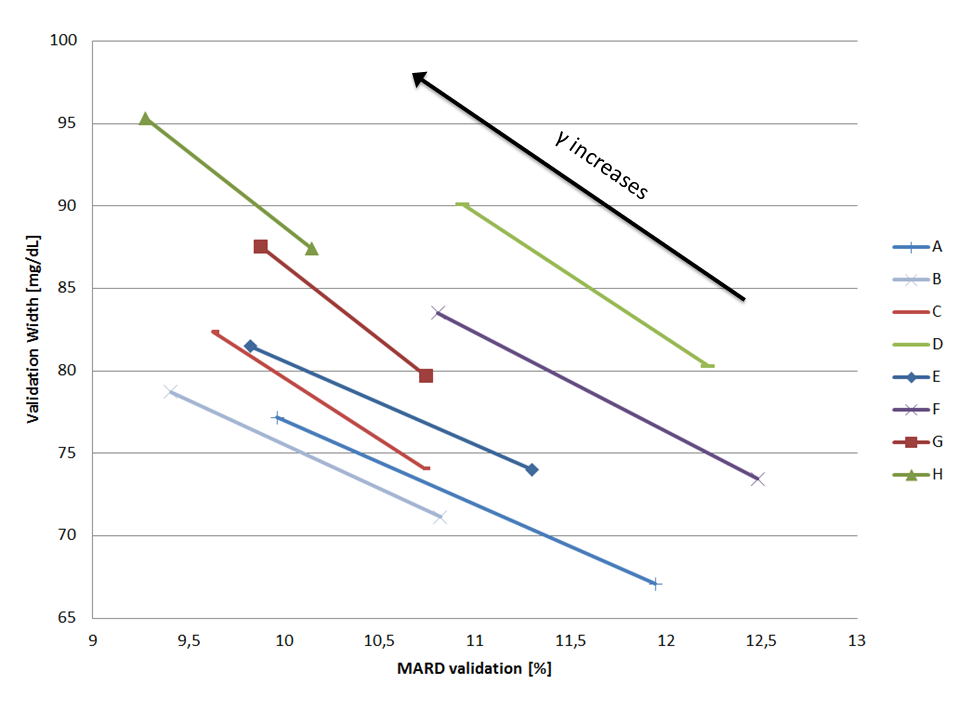
\epsfig{file=Figures/YSISCInsscenarios.png, width=\textwidth}\caption{Representation of the validation space of the results for the identification of all the scenarios considered. Two identifications for different $\gamma$ value are displayed, and the approximate direction of the $\gamma$ increment is plotted.}
\label{fig:YSISCInsscenarios}
\end{figure}

It is clear that some combinations of parameters yield better predictions than others. $\gamma$ gradient clearly displaces the validation results towards the top left direction, even though the results displayed do not correspond to the direct application of the weighting index, but rather the validation of those. Out of each pair of points in the graph, the top left point correspond to the $\gamma=100$ experiment of each identification scenario, and the $\gamma=50$ is located in the bottom right of the pair. It is worth noting that two points hardly define a pareto front and as such, no assumptions of the optimality of one scenario or the other must be taken by looking at the pair of points as a whole. Each scenario, taking into account the parameter vector identified and $\gamma$ must be regarded separately for the selection of a better case in the full model identification paradigm. 

Scenario B seems at a first glance to be closer to the ideal solution than the rest of the scenarios (being the ideal solution the best of both objectives for all the individuals). However, this scenario presents a much larger env\_fit value than the other solutions close to the ideal (mean env\_fit B100>A100; 18.73>16.24; p<0.005 and B100>C100; 18.73>16.95; p=0.041). Other solutions close to the ideal point are the scenarios A and C. All of these cases include the identification of the parameter $\alpha$, thus reinforcing the hypothesis drawn in the in-patient study on the importance of this parameter.

The ruled out scenario B considers the newly introduced parameter $\beta$ for the identification of the subcutaneous insulin subsystem. This parameter is identified in almost every patient and permutation to the optimization boundary, hinting a problem with identifiability even though the formal identifiability analysis proved it sensible for identification. This problem with parameter $\beta$ is not only a matter of scenario B; scenario A, which also identifies parameter $\beta$, identifies this aggregated parameter to the optimization boundary 87\% of the experiments. Simulations of the identified sets of parameters proved that plasma insulin levels were being identified too low for the data available.

In order to finally discard scenario A from identification feasibility, a comparison to the competing scenarios is to be performed on the prediction capabilities. Envelope width for the validation days is smaller of the scenario A100 (77,1 mg/dL) than in scenario C100 (82,4 mg/dL) with a significance p<0.005. However, no difference in the envelope fitness is appreciated (mean env\_fit A100=16.24>C100=16.95 p=0.078) meaning that no overestimation is assigned into the width difference. Also, MARD values are very similar, with no significance (p=0.226) on the error of the scenario C100 being better than scenario A100. 

Scenario C50 can be also taken into consideration as the optimal solution. Every comparison of the metrics of validation for the identifications results statistical significant when comparing same parameter vectors but different $\gamma$ values. Therefore scenario C50 can be compared to scenario C100 taking into account that envelope fitness and widths of the simulations of the validation days is lower, but the MARD and predicted samples are worse. A $\gamma$ value of 100 is preferred for the sake of coherence with the in-patient study since the same reference glucose data is used (being equally trustful), where the weighting factor was the same, and considering that the quality of the fitting data is the same, an equal value of $\gamma$ is preferred for comparison purposes.

Considering finally scenario C100, prediction capabilities are very good, with an average MARD of 9.63\% (median 4.34\%). These MARD values are consistent with the previous findings an represent a degree of error equal or lower than those of CGM devices currently in the market. gMARD metric for scenario C100 displays an average of 11.24\% (median 4.59\%) posing relatively small danger to the patient.

Using scenario C100, patients that were considered good identifications on the in-patient study do not behave so well in the case of introducing the subcutaneous insulin subsystem. That is the case of patient 9, which was reported as an example of good identification independently of the permutations in the in-patient study, but when plasma insulin is removed of the identification it does not work so well. Patient 9 identification is shown in Figure \ref{fig:ysiscinspatient9}.

\begin{figure}[hbt]
\centering
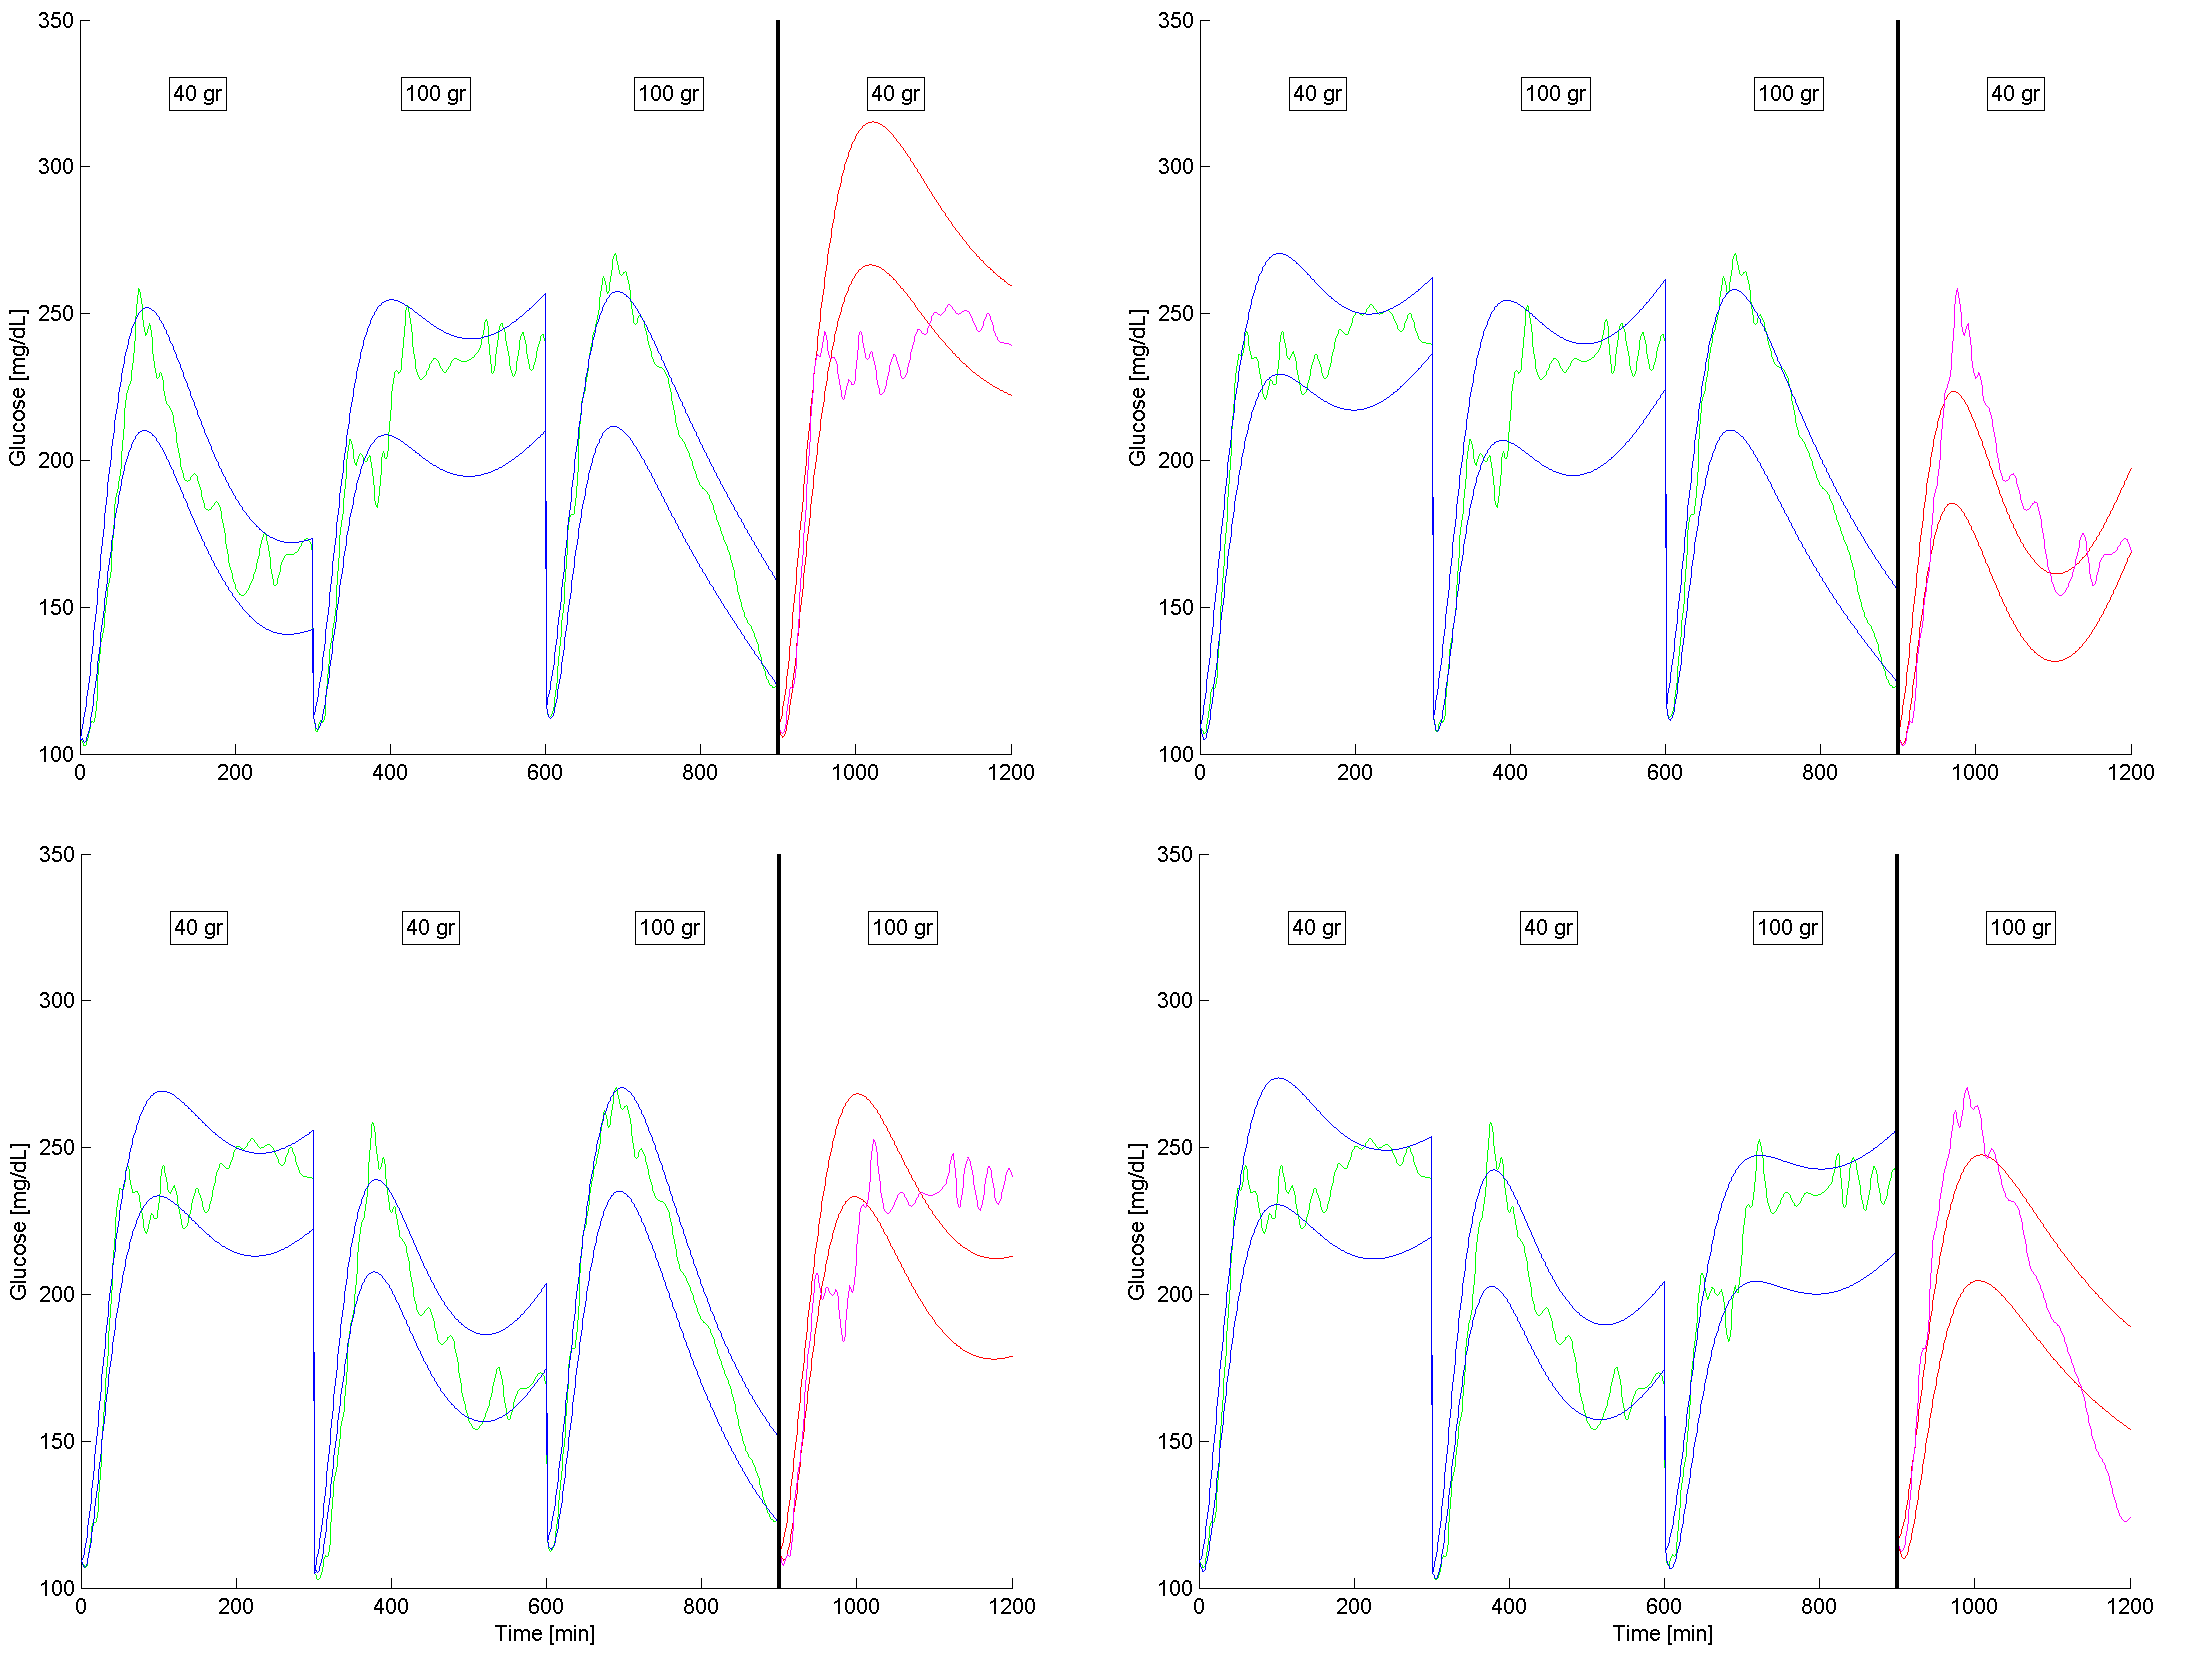
\epsfig{file=Figures/YSISCINSpatient_9.png, width=\textwidth}\caption{Patient 9 identification and validation results for the scenario C100. Day 1 validation is shown top left. Top Right graph shows validation for day 2. Bottom left validates day 3. Bottom right shows validation for day 4.}
\label{fig:ysiscinspatient9}
\end{figure}

By looking at the permutations of patient 9, it can be clearly seen that plasma insulin dynamics in the in-patient study contained information for the identification of glucose that helped the model to predict the patient easier. The subcutaneous model of insulin absorption can simulate very simple dynamics (even with uncertainty), but physiology of the subcutaneous route is more complex. Loss of predictability with respect to the in-patient study is attributed to this unmodelled dynamics.

Nevertheless, patient predictability is considered acceptable in most of the patients. In Figure \ref{fig:ysiscinspatient1}, simulation of all the permutations available for patient 1 are displayed.

\begin{figure}[hbt]
\centering
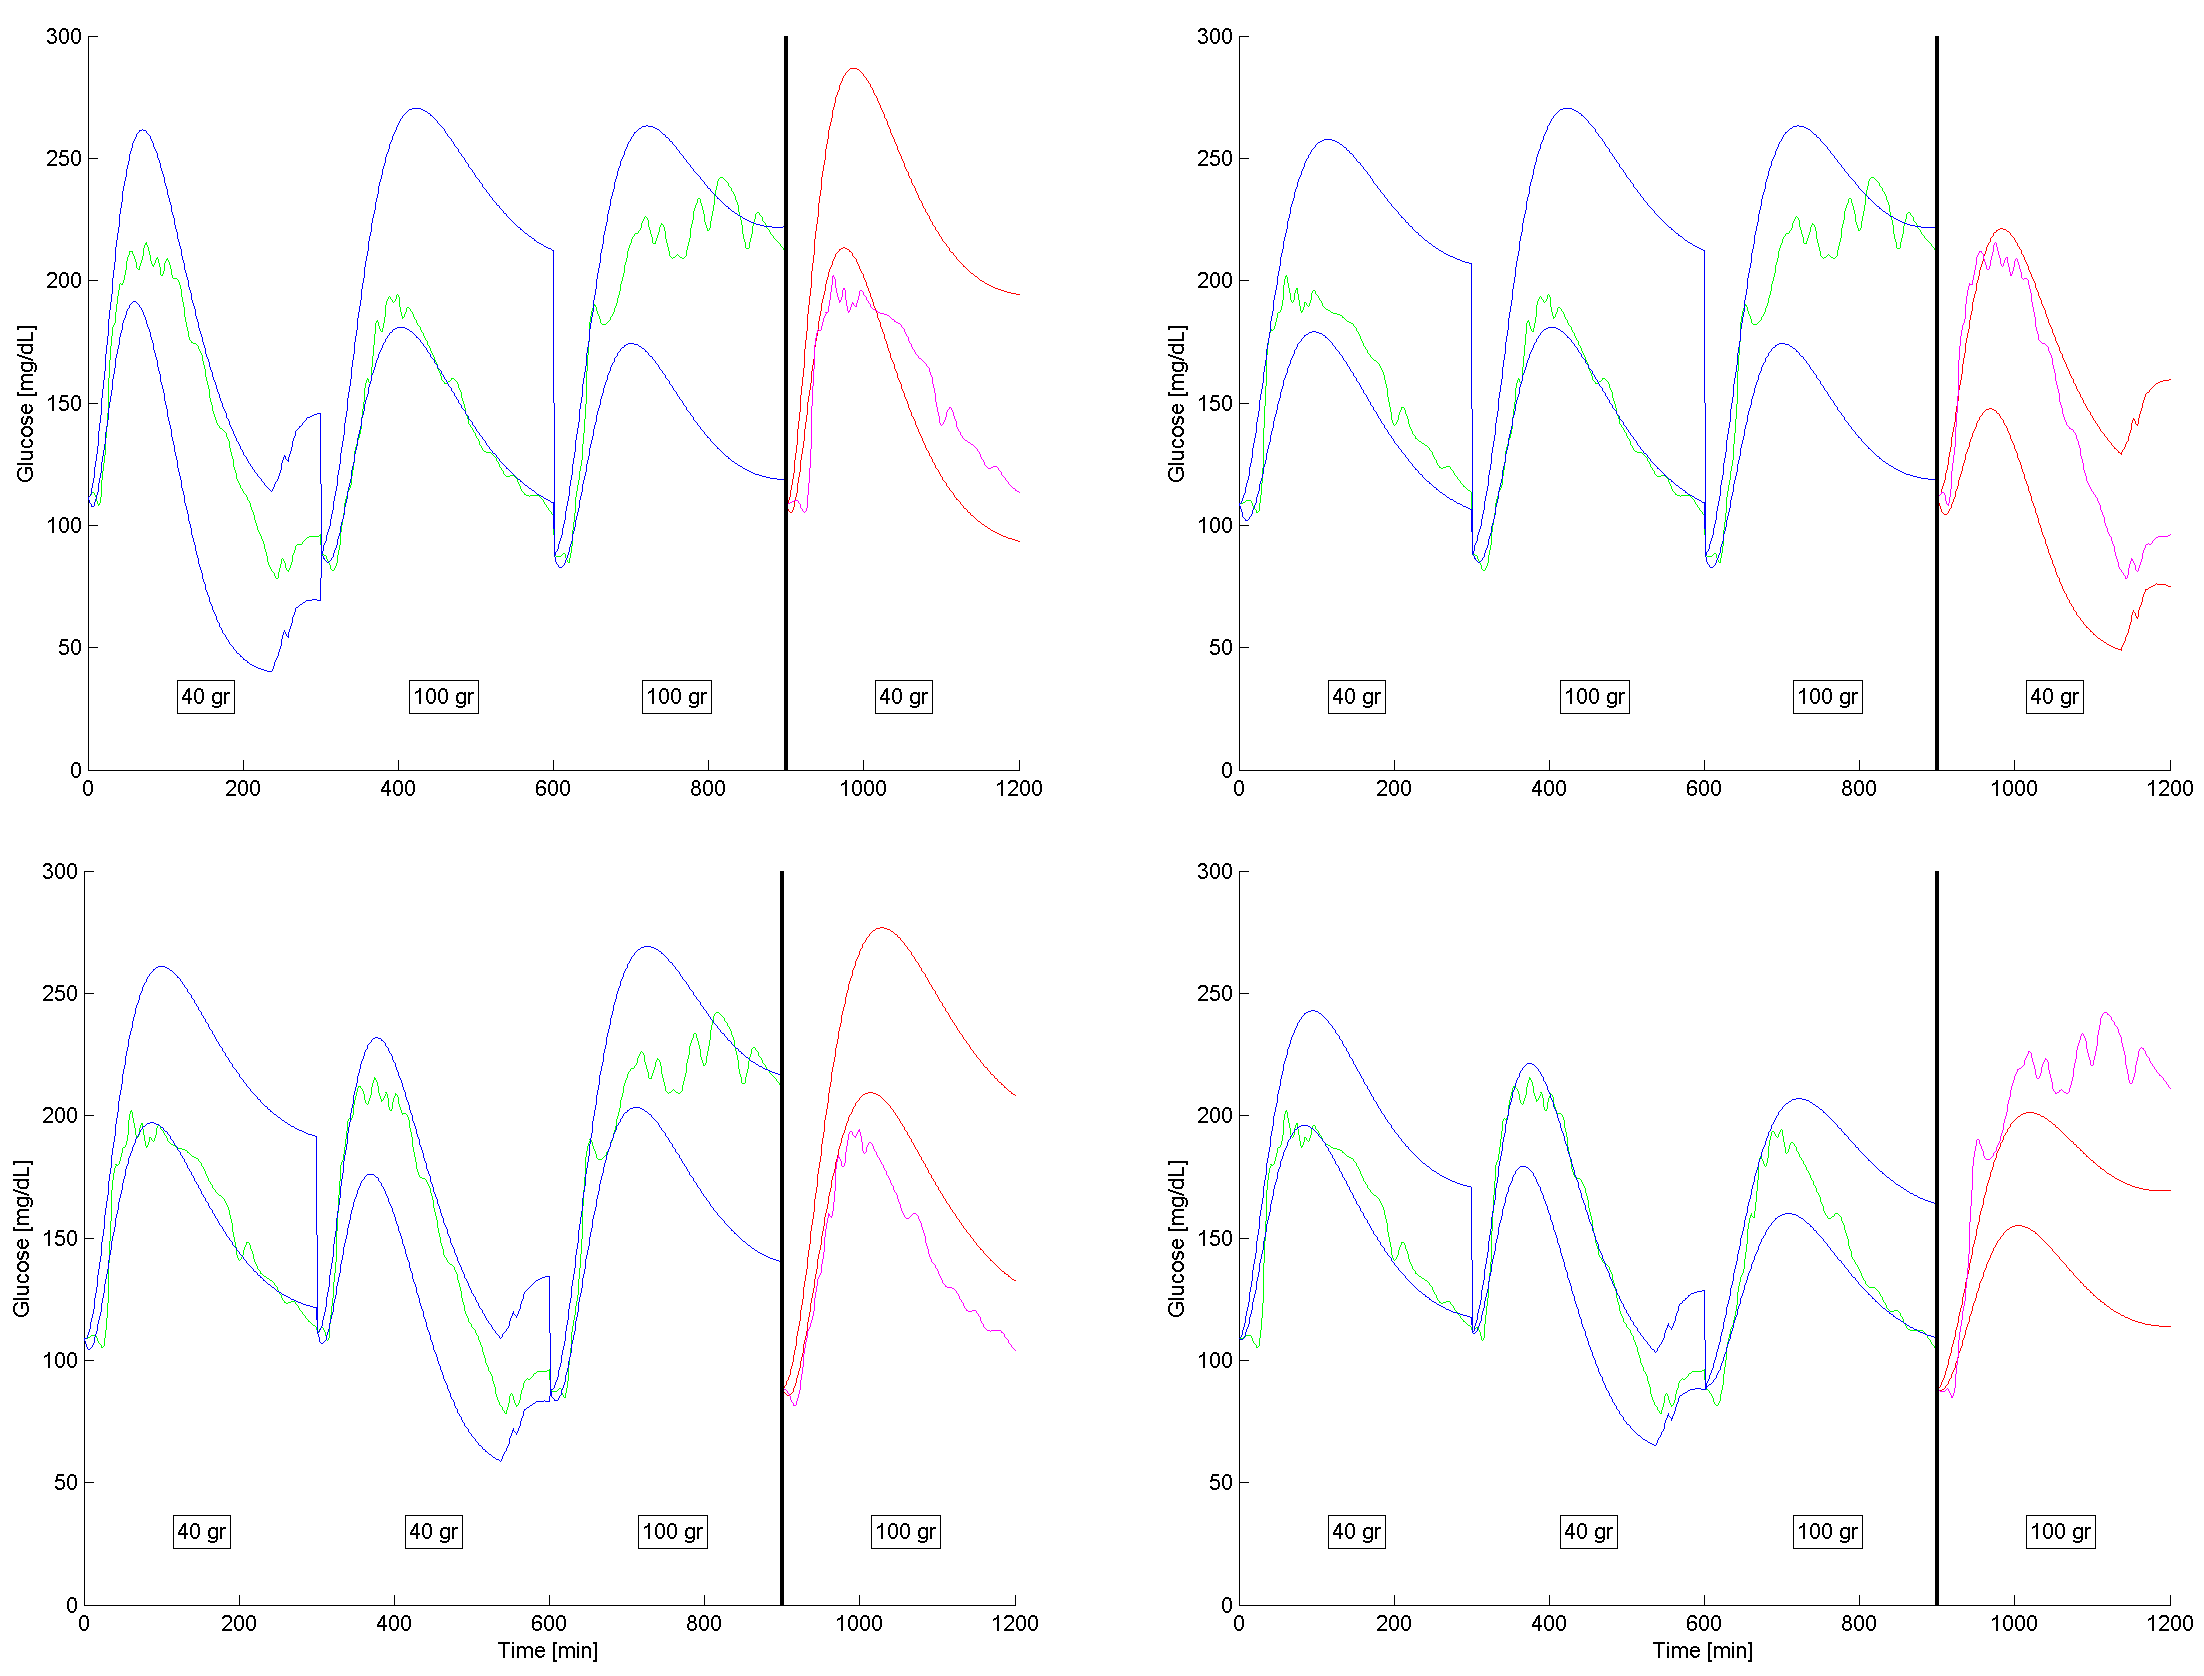
\epsfig{file=Figures/YSISCINSpatient_1.png, width=\textwidth}\caption{Patient 1 identification and validation results for the scenario C100. Day 1 validation is shown top left. Top Right graph shows validation for day 2. Bottom left validates day 3. Bottom right shows validation for day 4.}
\label{fig:ysiscinspatient1}
\end{figure}

Patient 1 is considered to be an average case of identification for this set of identifications. Two of the permutations show very good prediction capabilities, validating day 1 and day 2. The other two permutations fail at capturing the full variability of the patient and over (day 3) or underestimate (day 4) the postprandial response of the patient almost completely. The identification performed using the second permutation is considered the best case for this patient.

Best cases metrics of all the scenarios are presented in Table \ref{tab:resultsbestcaseYSISCINS} (for validation days). Best cases are calculated by selecting the best gMARD permutation for each patient.

\begin{table}[hbt]
	\centering
	\begin{tabular}{| c | c | c | c | c | c | c | c | c | c |} 
	\hline
	\multicolumn{2}{|c|}{Scenario} & A & B & C & D & E & F & G & H \\											
	\hline
	\multicolumn{10}{|c|}{$\gamma = 100$} \\
	\hline
	env\_fit & mean & 17.8 & 23.8 & 21 & 21.3 & 19.7 & 22 & 21 & 22.9 \\
	(mg/dL) & median & 18.4 & 17.6 & 19.7 & 17.3 & 18.7 & 18.4 & 20.9 & 18.9 \\
	\hline
	Width & mean & 93.6 & 107.8 & 114.5 & 112.4 & 100.2 & 102 & 104.6 & 113 \\
	(mg/dL) & median & 93.2 & 95.6 & 99.1 & 113 & 97.1 & 103.7 & 98.9 & 120.9 \\
	\hline
	Pred. & mean & 77.7 & 83.6 & 84.6 & 82.6 & 82.8 & 86.8 & 87.8 & 85.9 \\
	(\%) & median & 86.2 & 88.2 & 94.5 & 91.3 & 89.5 & 92.3 & 92.8 & 88.8 \\
	\hline
	MARD & mean & 1.26 & 0.96 & 1.25 & 1.25 & 0.83 & 0.83 & 0.66 & 0.73 \\
	(\%) & median & 0.65 & 0.46 & 0.11 & 0.53 & 0.46 & 0.29 & 0.12 & 0.28 \\
	\hline
	gMARD & mean & 1.43 & 0.99 & 1.27 & 1.28 & 0.89 & 0.84 & 0.73 & 0.8 \\
	(\%) & median & 0.72 & 0.5 & 0.11 & 0.58 & 0.48 & 0.29 & 0.12 & 0.29 \\
\hline
\multicolumn{10}{|c|}{$\gamma = 50$} \\
\hline
	env\_fit & mean & 16.7 & 19.4 & 18.4 & 19.7 & 19.6 & 19.3 & 19.4 & 20.9 \\
	(mg/dL) & median & 16.3 & 15.2 & 16.3 & 15.5 & 18.5 & 15.7 & 19.4 & 17.8 \\
	\hline
	Width & mean & 83.4 & 89.8 & 99.3 & 100.9 & 94.7 & 94.8 & 96.6 & 105.3 \\ 
	(mg/dL) & median & 85.2 & 85.6 & 90.5 & 98.4 & 93 & 96.7 & 94.3 & 111.6 \\
	\hline
	Pred. & mean & 72.2 & 79.4 & 79.6 & 74.1 & 81.9 & 82.1 & 84.9 & 82.8 \\
	(\%) & median & 83.2 & 86.8 & 85.5 & 85.7 & 86.7 & 87.2 & 92 & 86.7 \\
	\hline
	MARD & mean & 1.81 & 1.35 & 1.6 & 1.96 & 0.99 & 1.05 & 0.91 & 0.99 \\
	(\%) & median & 0.85 & 0.68 & 0.75 & 0.78 & 0.59 & 0.55 & 0.21 & 0.57 \\
	\hline
	gMARD & mean & 1.91 & 1.42 & 1.61 & 2.02 & 1.08 & 1.18 & 0.98 & 1.10 \\
	(\%) & median & 1.05 & 0.83 & 0.81 & 0.79 & 0.67 & 0.55 & 0.22 & 0.63 \\
\hline
	\end{tabular}
\caption{Results for all the scenarios for best case permutation of each patient.}
\label{tab:resultsbestcaseYSISCINS}
\end{table}

As it happened with the in-patient study, there is always a minimum of one permutation per patient that predicts with accuracy the validation day postprandial response. Best cases statistics are calculated from the 12 best days of the 12 patients under study, and being a small population, they are much more sensible to outliers. Despite this fact, it can be observed again that widths are always larger for the best case of each scenario than for the full cross-validation study. gMARD is obviously smaller since it is the decision metric to select each permutation to be the best case. MARD is also very small, at around 1\% error for every scenario.

A representative case of the best case permutation is presented in Figure \ref{fig:ysiscinspatient6}.

\begin{figure}[hbt]
\centering
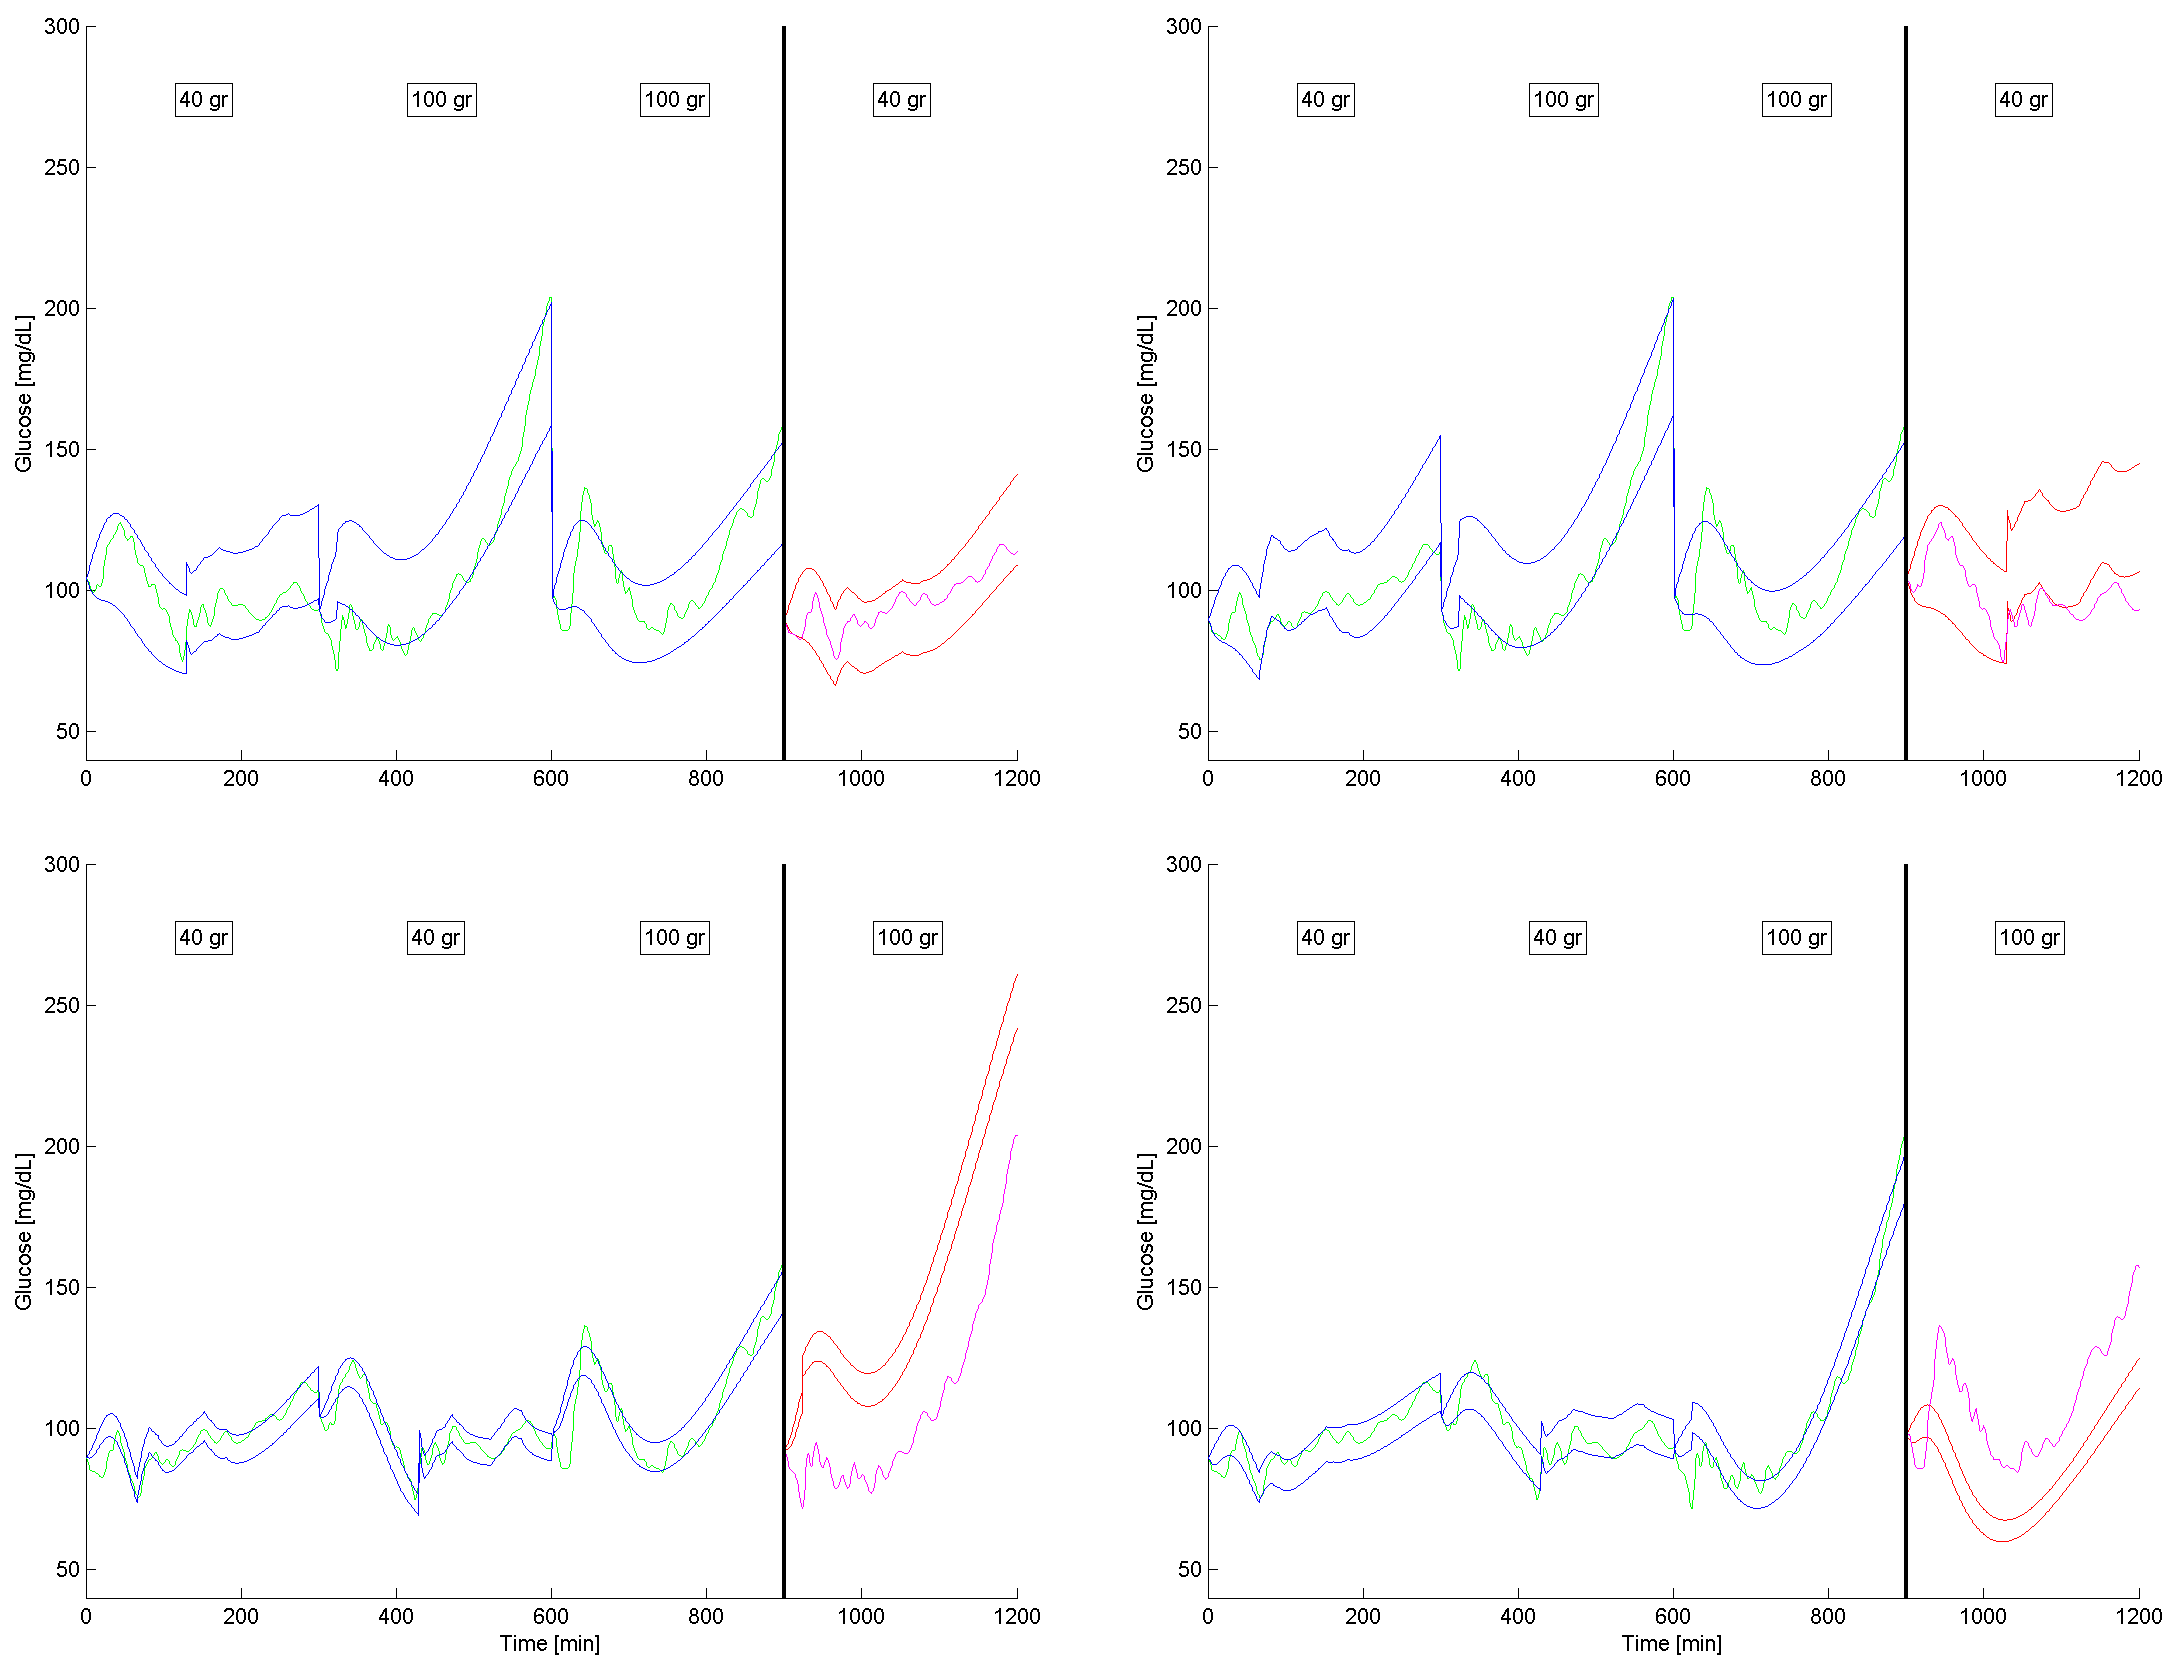
\epsfig{file=Figures/YSISCINSpatient_6.png, width=\textwidth}\caption{Patient 6 identification and validation results for the scenario C100. Day 1 validation is shown top left (best case). Top Right graph shows validation for day 2. Bottom left validates day 3. Bottom right shows validation for day 4.}
\label{fig:ysiscinspatient6}
\end{figure}

In patient 6 case only 1 day is well validated while the rest of days show no prediction capabilities. Note that patient 6 presented tendency to hypoglycemia at the moment of the monitoring, and IV glucose infusion was delivered in days 1 and 2. This intravenous glucose infusion prevented the patient to go into hypoglycemia but introduced a new perturbation to be modeled and identified. While the choice of this hypoglycemia prevention method was to use IV glucose infusion in order to minimize the influence of further glucose absorption dynamics (e.g intestinal absorption), the endogenous model still may use this information in the parameter tuning routine. This is the case on the validation of day 2, where glucose infusion was delivered throughout the whole postprandial period. If this infusion is left out of the identification days, as in the second permutation, the validation is much more difficult than in case of including this information, as happens in permutation 1, even though envelope validation widths may be larger (validation width permutation 1 = 32 mg/dL vs 39.2 mg/dL in permutation 2). Also, days 3 and four represent clearly the extremes of variability of the patient, given that when both are included in the identification set, the width is much larger.

The hypothesis of best cases introduced in the in-patient study seems to be valid in this case as well. MARD in the best cases is virtually zero and there is no difference between scenario. Concerning scenario C100, which has been chosen as the optimal parameter set, widths associated to the best case are larger (mean 114.5 mg/dL) than the widths for the whole dataset (mean 82.4 mg/dL) and this difference is significant with a factor p=0.0272. This does not translate however into a poor fitting of the identification data, since envelope fitness is not significantly different in the best case set and in the whole dataset (mean best case env\_fit=21 > cross-validation env\_fit=17; p=0.074). gMARD difference for the best cases in comparison to the MARD is virtually non-existent, posing these identification no danger to the patient's safety.

The number of patients available is a very important issue and should be focus of the discussion in this type of analysis. It is clear that 12 patients is hardly enough to draw conclusions in a matter that affect very large populations, as is the case of diabetes modeling. It is very difficult however to find datasets open for research groups to access and experiment with. The reason for this conservative behavior from large research groups is of course that gathering real patient data from type 1 diabetic patients is extremely difficult and costly. Considering different sample sizes, some of the treats exposed in this thesis may become significant where now are not, or viceversa.

However, interval identification poses a major tool for characterization of patient's postprandial behavior, even when great difficulties are tested against it such as the uncertainties of daily life in a diabetic patient, or the lack of reliable models for subcutaneous insulin infusion. This methodology is yet to be tested to one of the greatest difficulties in the process of diabetes modeling: the continuous glucose monitor signals, which will be accounted for in the following lines.

\section{Identification from CGM data}
\label{sec:CGMIdentification}

CGM error has been proven significant in the measurements of glucose, and ultimately one of the main problems in full patient identification in diabetes. Previous efforts were performed on this thesis in the analysis and modeling of the error signal produced by this type of devices (see Chapter \ref{sec:CGMStatisticalModelingAndValidation}), proving very useful for simulation purposes and for virtual identification studies. The same CGM signals used for the deduction of the models for the Dexcom\textsuperscript{\textregistered} SEVEN\textsuperscript{\textregistered} PLUS and the Medtronic\textsuperscript{\textregistered} Paradigm\textsuperscript{\textregistered} Veo\texttrademark{} were included in the patients dataset for the final identification procedure.

By default the signal from the SEVEN\textsuperscript{\textregistered} PLUS monitor was used for the identification of the whole dataset, given that there were more postprandial periods provided by this monitor than with the Paradigm\textsuperscript{\textregistered} Veo\texttrademark{}, and also regarding at the results of the error analysis performed before, where the monitor from Dexcom provided significantly better glucose estimations for this particular dataset.

Data fitting methodology is exactly the same as in the works with YSI reference glucose measurements. From all the scenarios considered in the previous chapter, only the settings of scenario C are used for CGM data fitting, given that the results with YSI hinted a superior capacity of prediction of data samples than in the other configurations. The final set of parameters identified, separating the interval parameters as their upper and lower bounds, is as follows:
\begin{equation}\label{eq:parametervectorCGMscenarioC}
\begin{split}
\theta=&[\underline{S_{iT}}, \overline{S_{iT}}, \underline{S_{iD}}, \overline{S_{iD}}, \underline{S_{iE}}, \overline{S_{iE}}, \underline{k_{12}}, \overline{k_{12}}, \underline{k_e}, \overline{k_e}, \underline{\alpha}, \overline{\alpha}, \\
& t_{maxI}, t_{maxG40}, t_{maxG100}, V_g ]
\end{split}
\end{equation}
The total number of optimization variables is 16, including 6 interval parameters. Initial interval glucose is not identified, despite the uncertainty introduced by the CGM, due to the fact that only CGM measurements are used to fit the data. If uncertainty was introduced to the initial glucose of the identified model, the fitting algorithm would force the interval to resemble the CGM measurement as much as possible (as CGM is the only available information available to the algorithm), leading to low uncertainty in the initial condition. If uncertainty was included in the initial glucose of the simulation, it would have to be added \textit{a priori}. This \textit{a priori} uncertainty in the initial conditions may be a focus of study in the future, but it is not considered here for the sake of simplicity of the identification problem. 

The weighting factor $\gamma$ of the identification index is considered to be an estimation of the researcher of the confidence that is entrusted in the data used for the fitting. CGM is known to introduce significant errors in the glucose profiles of diabetic patients, especially in the postprandial period, and this is logically translated in a mistrust attitude to this type of data. $\gamma$ is then supposed to be lower than the values used for the identification of YSI data, but the values to be used is not known. In here, 6 different values of $\gamma$ are considered in order to create an approximately continuous front in the pareto space from where to extract a desired scenario which related to a defined $\gamma$ value. The six values of $\gamma$ are, decreasing from the value of the YSI identification: 100, 85, 70, 55, 40, 25.

CGM influence on the identification experiment is enormous. Out of the 12 patients available in the dataset, 2 were discarded due to CGM malfunctions. An example of CGM malfunction that nullifies the patient's identification is displayed in figure \ref{fig:patient7failCGM}, corresponding to patient 7.

\begin{figure}[hbt]
\centering
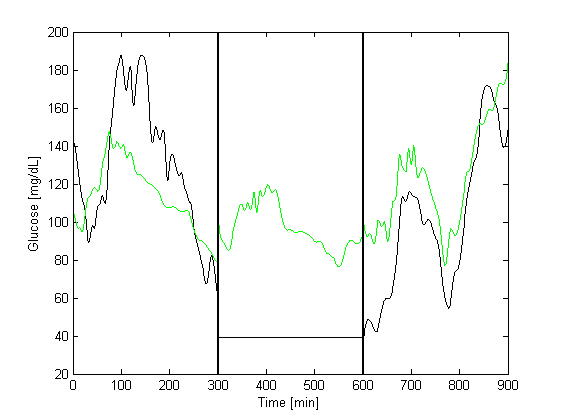
\epsfig{file=Figures/patient7failCGM.png, width=\textwidth}\caption{One of the permutations of patient 7 where two of the CGM monitoring signals are faulty at the beginning of the postprandial period. YSI signal is plotted in green and CGM estimation is plotted in black.}
\label{fig:patient7failCGM}
\end{figure}

Even though the CGM devices were calibrated before the experiment and new sensors were inserted the day before to the experiment, several cases of monitors starting the experiment in saturation levels are reported (lower saturation level = 40 mg/dL). Examples of this faulty behavior are patients 7, 9 and 11. All of these patients wore 2 different sets of CGM as explained before. Unfortunately, for patients 7 and 11 both monitors failed in the same days, yielding the data for those patients useless for the cross-validation study. These fails are in accordance to failure rate of these CGM devices, which can be up to 20\%. It is worth remembering that all the patients were successfully trained in the use of CGM and were long-term users of the insulin pump technology.

Patient 9 was saturated in one postprandial period for the Dexcom\textsuperscript{\textregistered} SEVEN\textsuperscript{\textregistered} PLUS monitor, but Medtronic\textsuperscript{\textregistered} Paradigm\textsuperscript{\textregistered} Veo\texttrademark{} performed correctly in that day. Patient 9 CGM data was modified to include the use of the Paradigm\textsuperscript{\textregistered} Veo\texttrademark{} in the identification for the postprandial period where the SEVEN\textsuperscript{\textregistered} PLUS failed. The final resulting set of patients is then reduced to 10.

The evaluation of the identifications is performed following the same metrics that were applied in the previous section, with different application focus. CGM signal is the data to be fit in the optimization process, and all the identification metrics and the identification composite index are evaluated in the CGM data of each patient. Therefore, performance of the methodology in the identification data for each permutation of the cross-validation study is applied to the corresponding CGM data. However, for prediction of the glucose behavior, it is the ``real'' blood glucose which wants to be predicted, not the CGM estimation. YSI data is thus the correct data to be used for the evaluation of the performance metrics in the validation days. It is worth noting that envelope fitness estimates makes more sense if evaluated to the same data used to fit, therefore the \textit{env\_fit} values are always reported on CGM data.

Computation cost on the CGM optimization was very similar to that of the YSI optimizations. Computation times for the algorithm used in this work are highly dependent on the number of parameters being tuned, and given that the number of parameters is fixed to 16, no difference between all the optimizations reported here is appreciated. Average optimization time was approximately 60 hours on a workstation Intel \textregistered Xeon \textregistered CPU 2.67 GHz with 4 GB of RAM memory running under Windows 7.

Results of the identification days for all the possible permutations are shown in Table \ref{tab:resultsCGMident}.

\begin{table}[hbtp]
	\centering
	\begin{tabular}{| c | c | c | c | c | c | c | c |} 
	\hline
	\multicolumn{2}{|c|}{$\gamma$} & 100 & 85 & 70 & 55 & 40 & 25 \\											
	\hline
	Width & mean &	104.8 & 102.4 & 99.5 & 94.1 & 88.2 & 76.4 \\
	(mg/dL) & median & 96.5 & 94.2 & 90.6 & 85.5 & 80.1 & 69.5 \\
	\hline
	Prediction & mean & 77.4 & 75.6 & 73.4 & 69.4 & 65.1 & 56.6 \\
	(\%) & median & 79.9 & 78 & 75.8 & 72.7 & 68.6 & 60.9 \\
	\hline
	MARD & mean & 1.24 & 1.37 & 1.59	& 2 & 2.53 & 3.69 \\
	(\%) & median & 1.11 & 1.24 & 1.43 & 1.74 & 2.31 & 3.34 \\
	\hline
	gMARD & mean & 1.67 & 1.85 & 2.16 & 2.73 & 3.44 & 4.93 \\
	(\%) & median & 1.49 & 1.67 & 2.07 & 2.39 & 3.21 & 4.65 \\
	\hline
	env\_fit & mean & 22.5 & 22 & 21.5 & 20.2 & 19 & 17.7 \\
	(mg/dL) & median & 21 & 20.2 & 19.2 & 18 & 16.1 & 15.9 \\
	\hline
\end{tabular}
\caption{Results for all the $\gamma$ values for the three identification days considering all possible permutations of days from the dataset.}
\label{tab:resultsCGMident}
\end{table}

Fitting statistics and envelope widths are worst than those obtained from YSI identification, as expected. When looking at the $\gamma=100$ case, for the sake of comparison, average width for the identification days goes from 86.9 mg/dL in the YSI identification in section \ref{sec:IdentificationFromReferenceGlucose3} to 104.8 mg/dL. \textit{env\_fit} is also worsened going from 17 mg/dL up to 22.5 mg/dL. This results in an overestimation of the width of the interval model, responding to the much inaccurate data source of the CGM. MARD is also larger (note that in identification data MARD is evaluated against CGM), going from 0.88\% of the YSI identification up to 1.24\%, even though prediction samples are very similar (YSI 77.3\% vs CGM 77.4\%).

Validation data is displayed in Table \ref{tab:resultsCGMval}.

\begin{table}[hbtp]
	\centering
	\begin{tabular}{| c | c | c | c | c | c | c | c |} 
	\hline
	\multicolumn{2}{|c|}{$\gamma$} & 100 & 85 & 70 & 55 & 40 & 25 \\											
	\hline
	Width & mean &	101.2 & 99.6 & 95.9 & 90.1 & 84.8 & 73 \\
	(mg/dL) & median & 91 & 84.5 & 85.6 & 79.6 & 73.9 & 62.4 \\
	\hline
	Prediction & mean & 61.1 & 60.7 & 58.4 & 54.8 & 54.5 & 48.3 \\
	(\%) & median & 69.3 & 67.8 & 62.5 & 57.7 & 61.8 & 49.7 \\
	\hline
	MARD & mean & 9.6 & 9.68 & 10.04 & 11.16 & 11.8 & 14.21 \\
	(\%) & median & 4.32 & 4.68 & 5.14 & 6.1 & 6 & 7.07 \\
	\hline
	gMARD & mean & 11.63 & 11.75 & 12.17 & 13.38 & 14.14 & 16.74 \\
	(\%) & median & 4.35 & 4.71 & 5.18 & 6.53 & 6.34 & 8.16 \\
	\hline
\end{tabular}
\caption{Results for all the $\gamma$ values for the validation day considering all possible permutations of days from the dataset.}
\label{tab:resultsCGMval}
\end{table}

Calculation of significance between the data of the CGM identifications and YSI identifications is not straightforward. Given that CGM identifications are only performed on 10 patients, paired permutation significance tests are not possible, unless the faulty CGM patients are removed from the YSI dataset. It is also possible to perform unpaired significance tests, but it is more reasonable to use the information available from the patient to perform the test. To do so, patients 7 and 11 are discarded, and the permutations tests performed as usual.

Validation widths for the $\gamma=100$ scenario of the CGM identification are larger than those of the identification with blood glucose reference (101.2 mg/dL > 82.4 mg/dL; p<0.005), but MARD values are very similar (YSI MARD = 9.63\% vs. CGM MARD = 9.6\%). Only $\gamma$ value of 100 is tested for this comparison, because it is the same as in the YSI experiment. Results for different $\gamma$ values are displayed in figure \ref{fig:CGMpareto} for easier visualization.

\begin{figure}[hbtp]
\centering
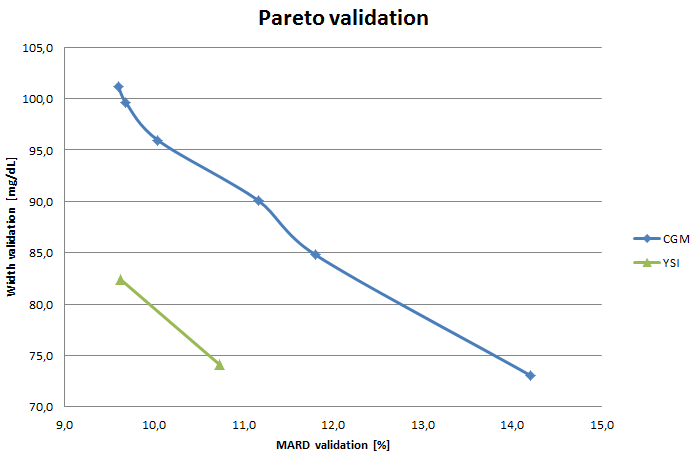
\epsfig{file=Figures/CGMpareto.png, width=\textwidth}\caption{Representation in the validation Pareto Space of the results for the identification of all the $\gamma$ values considered.}
\label{fig:CGMpareto}
\end{figure}

The range of $\gamma$ considered seems appropriate for the problem at stake, since the range covers from the same MARD level of the YSI identification (MARD=9.6\% at $\gamma$=100) up to very similar envelope widths from both identifications at $\gamma=25$ (YSI width 74.1 mg/dL vs CGM width 73 mg/dL). Looking at the whole set of identifications, $\gamma=70$ is closer in the pareto space to the much better solution that YSI identification poses than any other identification performed by CGM. Also, width decreases significantly from $\gamma=100$ to $\gamma=70$ for very similar MARD results, which makes this solution to be preferred. For lower $\gamma$ values, improvements on the envelope width come at the cost of dramatically increasing the average MARD for the whole dataset. All simulations onward are presented for the $\gamma=70$ scenario.

An example of identification with CGM is shown in figure \ref{fig:CGMpatient5}.

\begin{figure}[hbt]
\centering
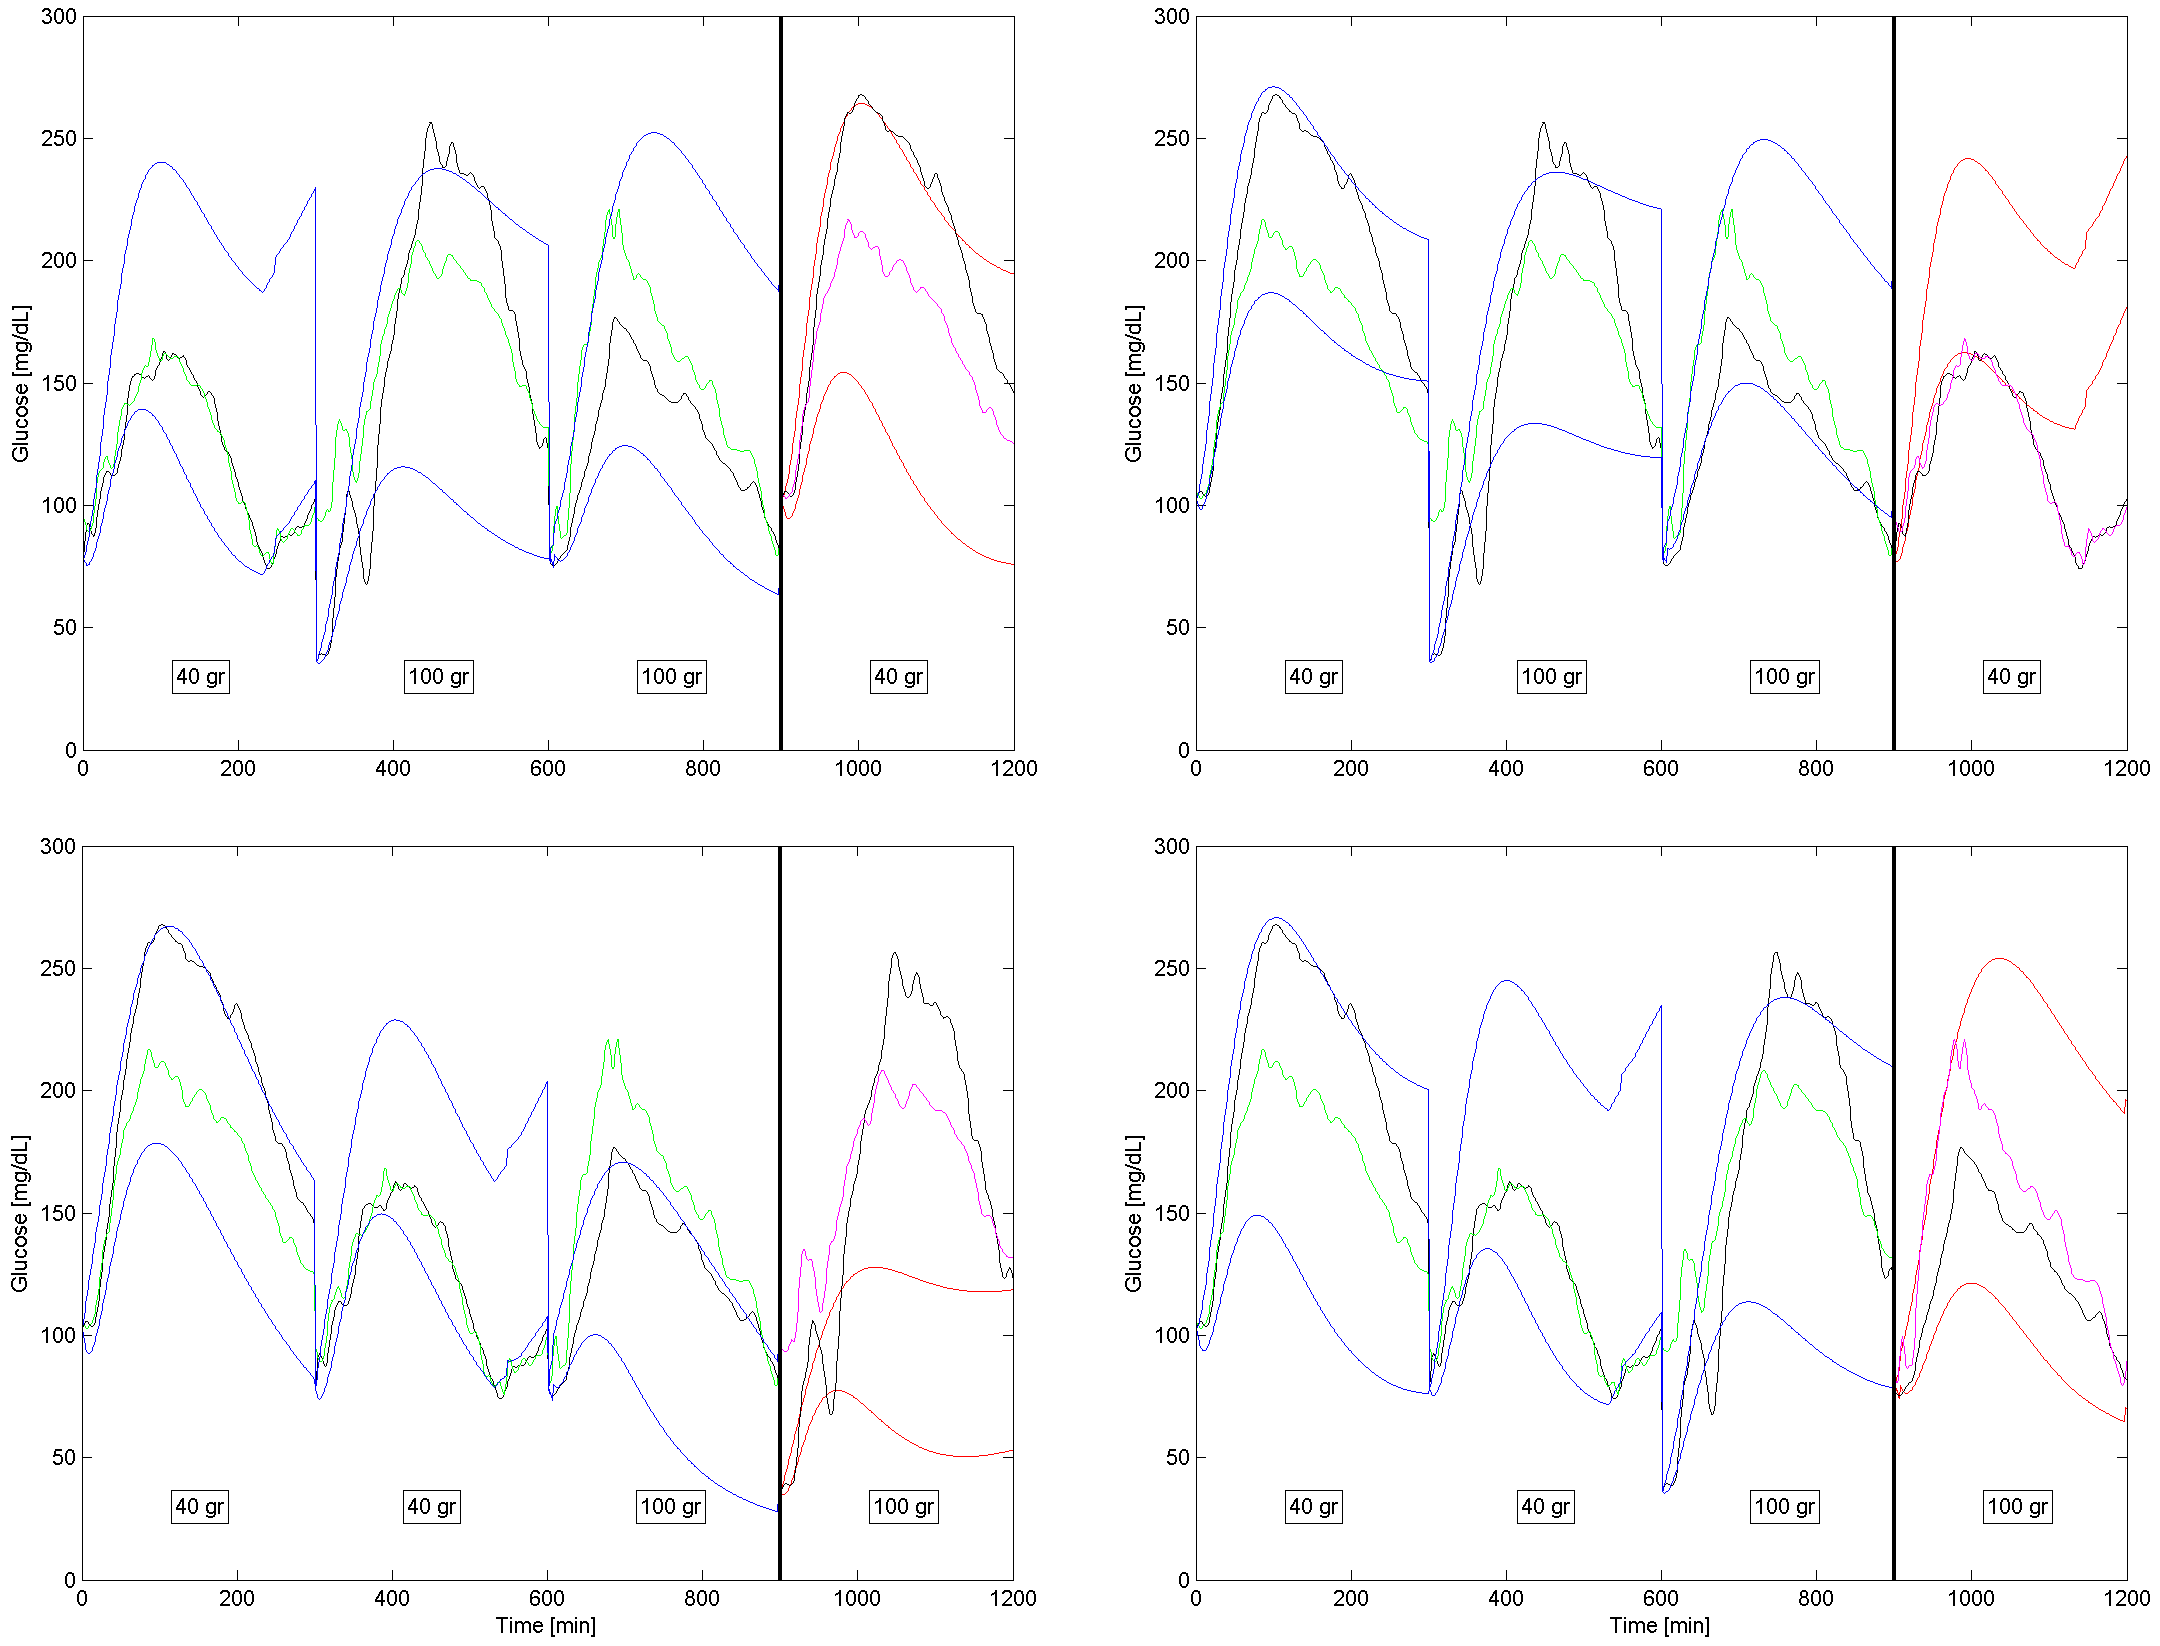
\epsfig{file=Figures/CGM_patient_5.png, width=\textwidth}\caption{Patient 5 identification and validation results for the scenario C100. Day 1 validation is shown top left. Top Right graph shows validation for day 2. Bottom left validates day 3. Bottom right shows validation for day 4. Black lines represent the CGM signal. YSI measurements are displayed in green for the identification days, and in magenta for the validation day.}
\label{fig:CGMpatient5}
\end{figure}

Patient number 5 shows very clearly the inconvenient of CGM identification. Even though the CGM was not considered faulty for the postprandial periods of this patient, several days present clear over or underestimations of the blood glucose signals. This behavior is very common on any CGM device and is part of the assumed error of the sensor's estimations. It does, however, affect greatly on the identifications performed. Disregarding the possibilities of inherent variability of the patient, it can be observed how overestimation of the signal causes the validation of the model to also overestimated the blood glucose reference signal. For example, in the validation of day 2 for patient 5, in two of the days used for identification the CGM rises approximately 50 mg/dL over the blood glucose reference, causing the envelope width to grow much larger and misplaced in the patient's average postprandial behavior. This problem is diminished in situations like the validation of day 1, where overestimation and underestimation occur in separate days of the identification set, causing the envelope width to be larger than required, but centered in the average postprandial behavior of the patient, thus including the validation data within the envelope. The larger envelopes identified in average for the CGM identification are explained by the performance of the identification of patient 5, which is a representative sample of an identification for this section.

Patient 9, for whom the Dexcom\textsuperscript{\textregistered} SEVEN\textsuperscript{\textregistered} PLUS monitor presented flat estimations, also is a very good example of identification with CGM. The identification performed for patient 9 is plotted in Figure \ref{fig:CGMpatient9}.

\begin{figure}[hbt]
\centering
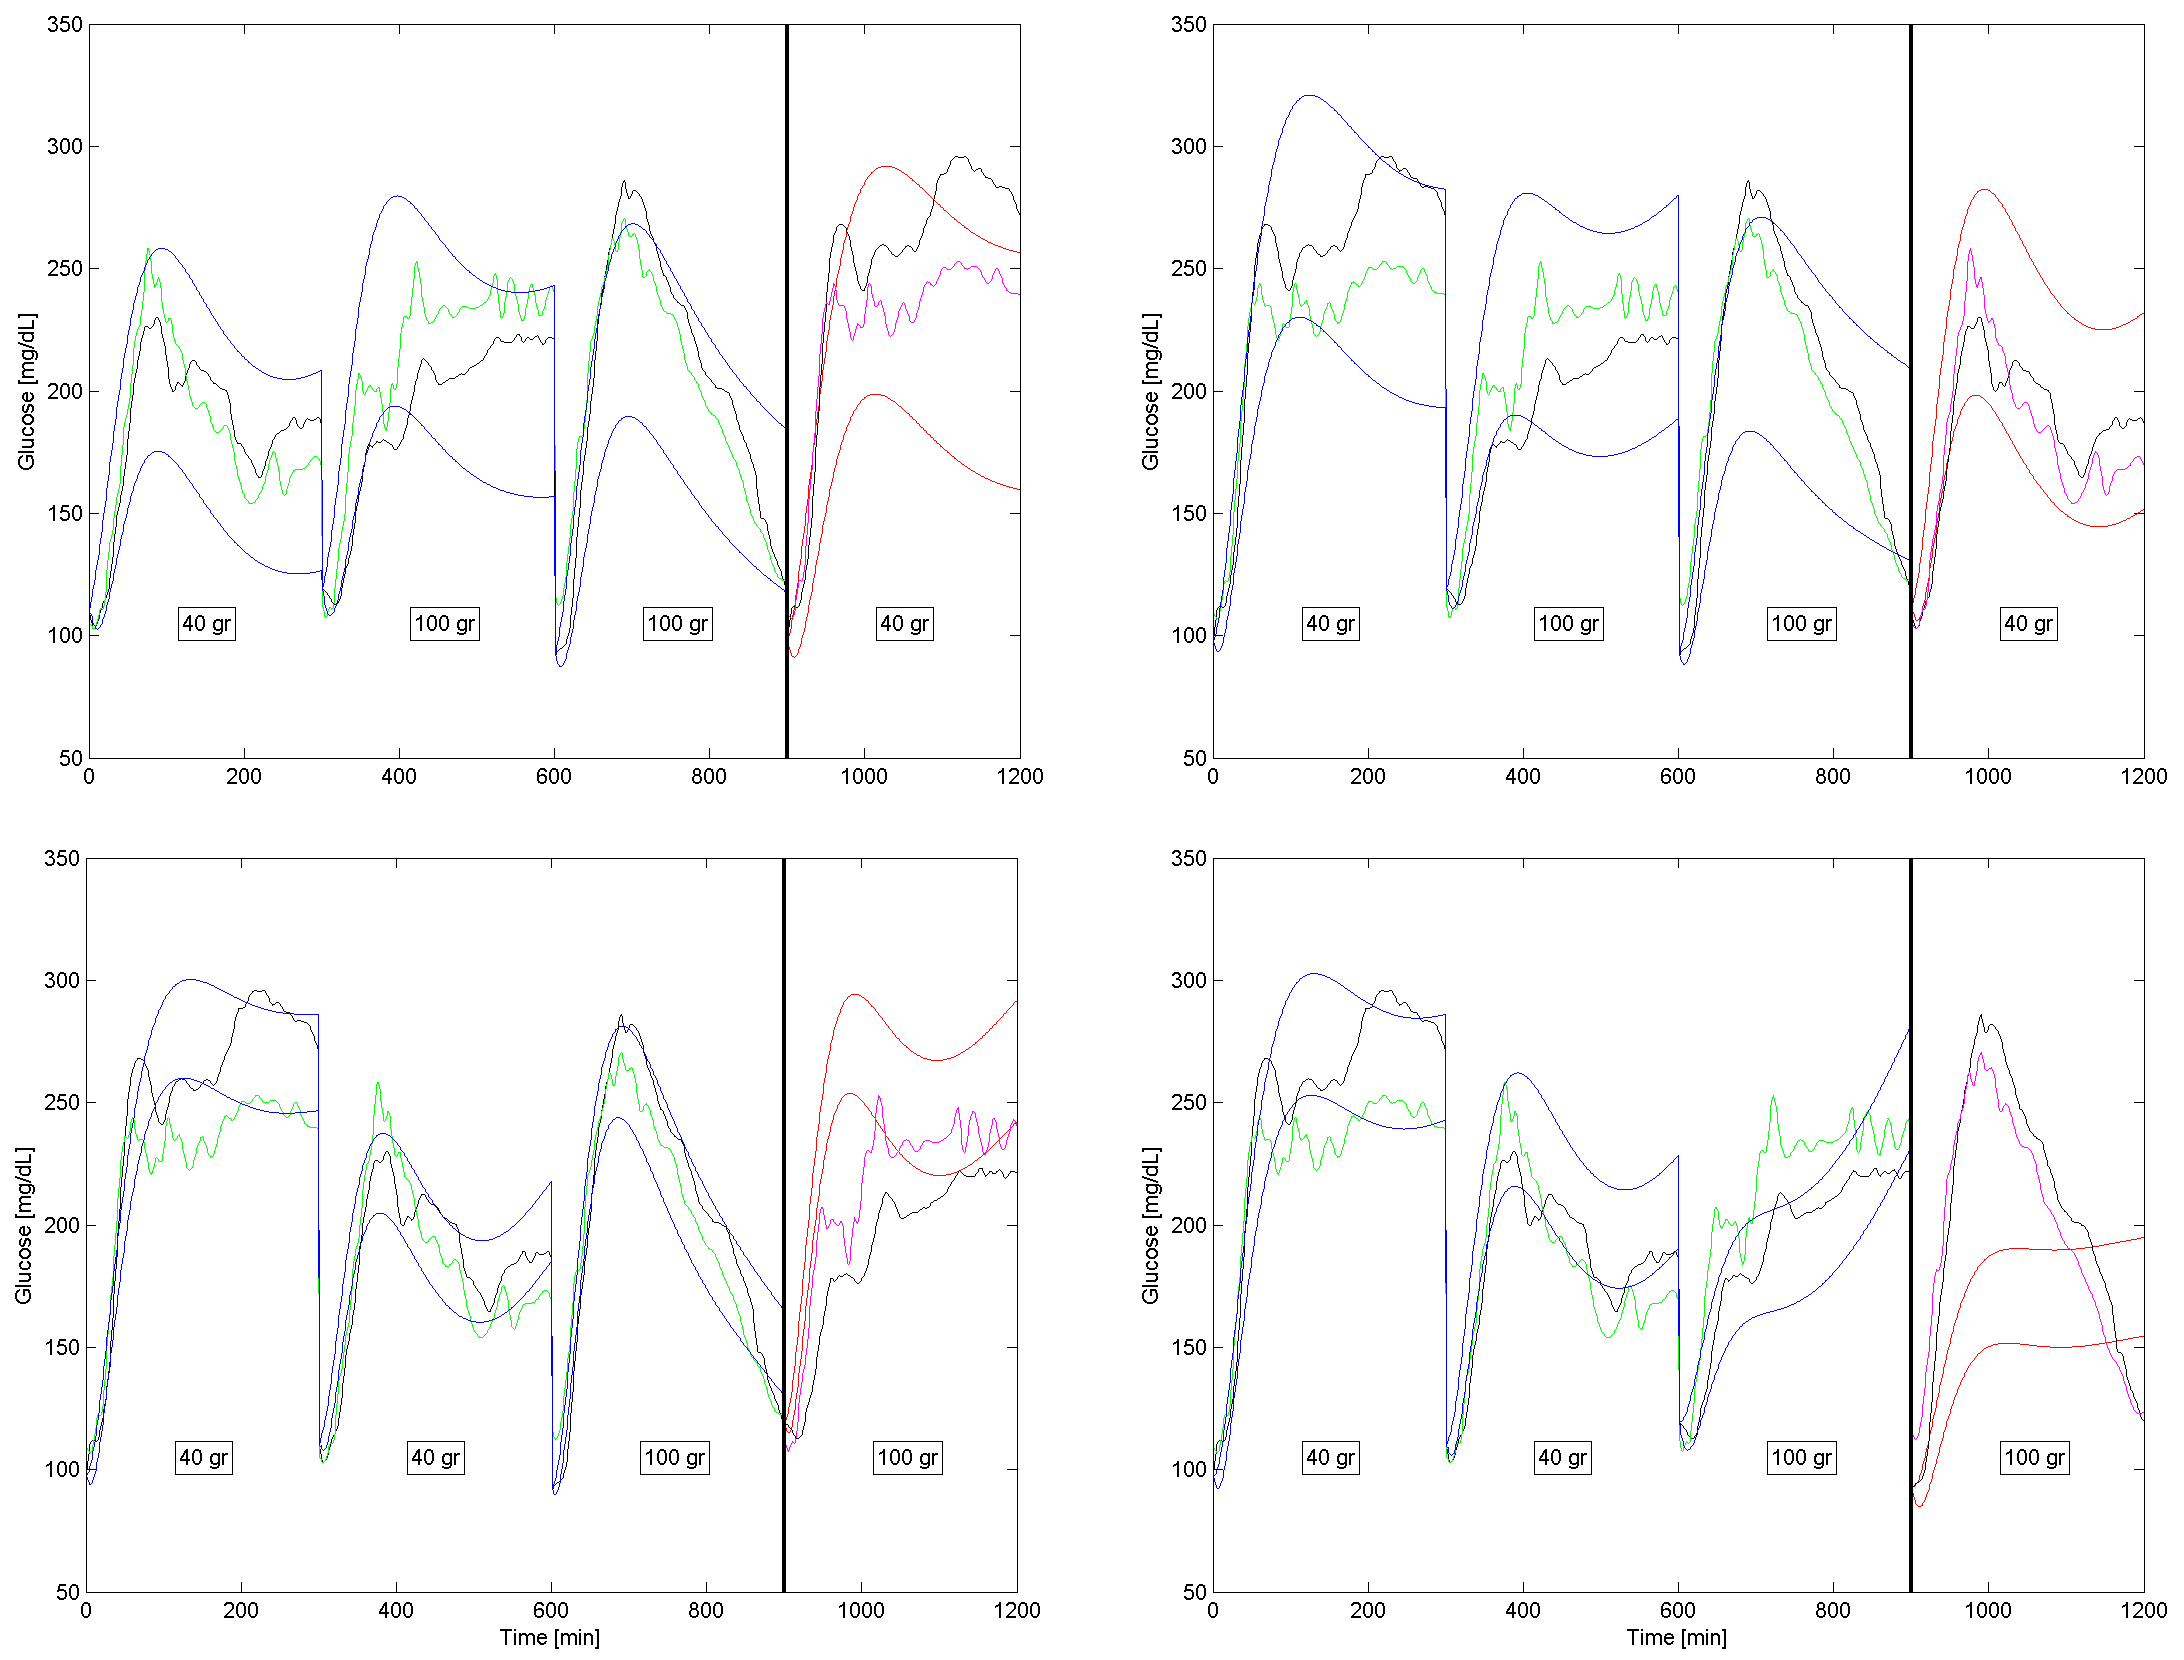
\epsfig{file=Figures/CGM_patient_9.png, width=\textwidth}\caption{Patient 9 identification and validation results for the scenario C100. Day 1 validation is shown top left. Top Right graph shows validation for day 2. Bottom left validates day 3. Bottom right shows validation for day 4. Black lines represent the CGM signal. YSI measurements are displayed in green for the identification days, and in magenta for the validation day.}
\label{fig:CGMpatient9}
\end{figure}

This patient supposes a good identification for all possible identifications paradigms: it was the best example of identification for the in-patient study, and although the introduction of the subcutaneous insulin model in the identification scenario worsened the outcome of the optimizations, it was yet a good example of identification with YSI for a full model of a patient. CGM performs reasonably well for this patient leading to a very similar performance in the identification to that obtained from YSI identification.

Permutations 1 and 2 (validation days 1 and 2) cover completely the validation data on the model's envelope. Permutation 3 does not present a good validation even though the data fitting is satisfactory. The last permutation represents a failed validation but also a poor fitting of the glucose signal in day 3 mostly caused by a bad CGM estimation.

The final example is patient 6, whose identification is displayed in figure \ref{fig:CGMpatient6}.

\begin{figure}[hbt]
\centering
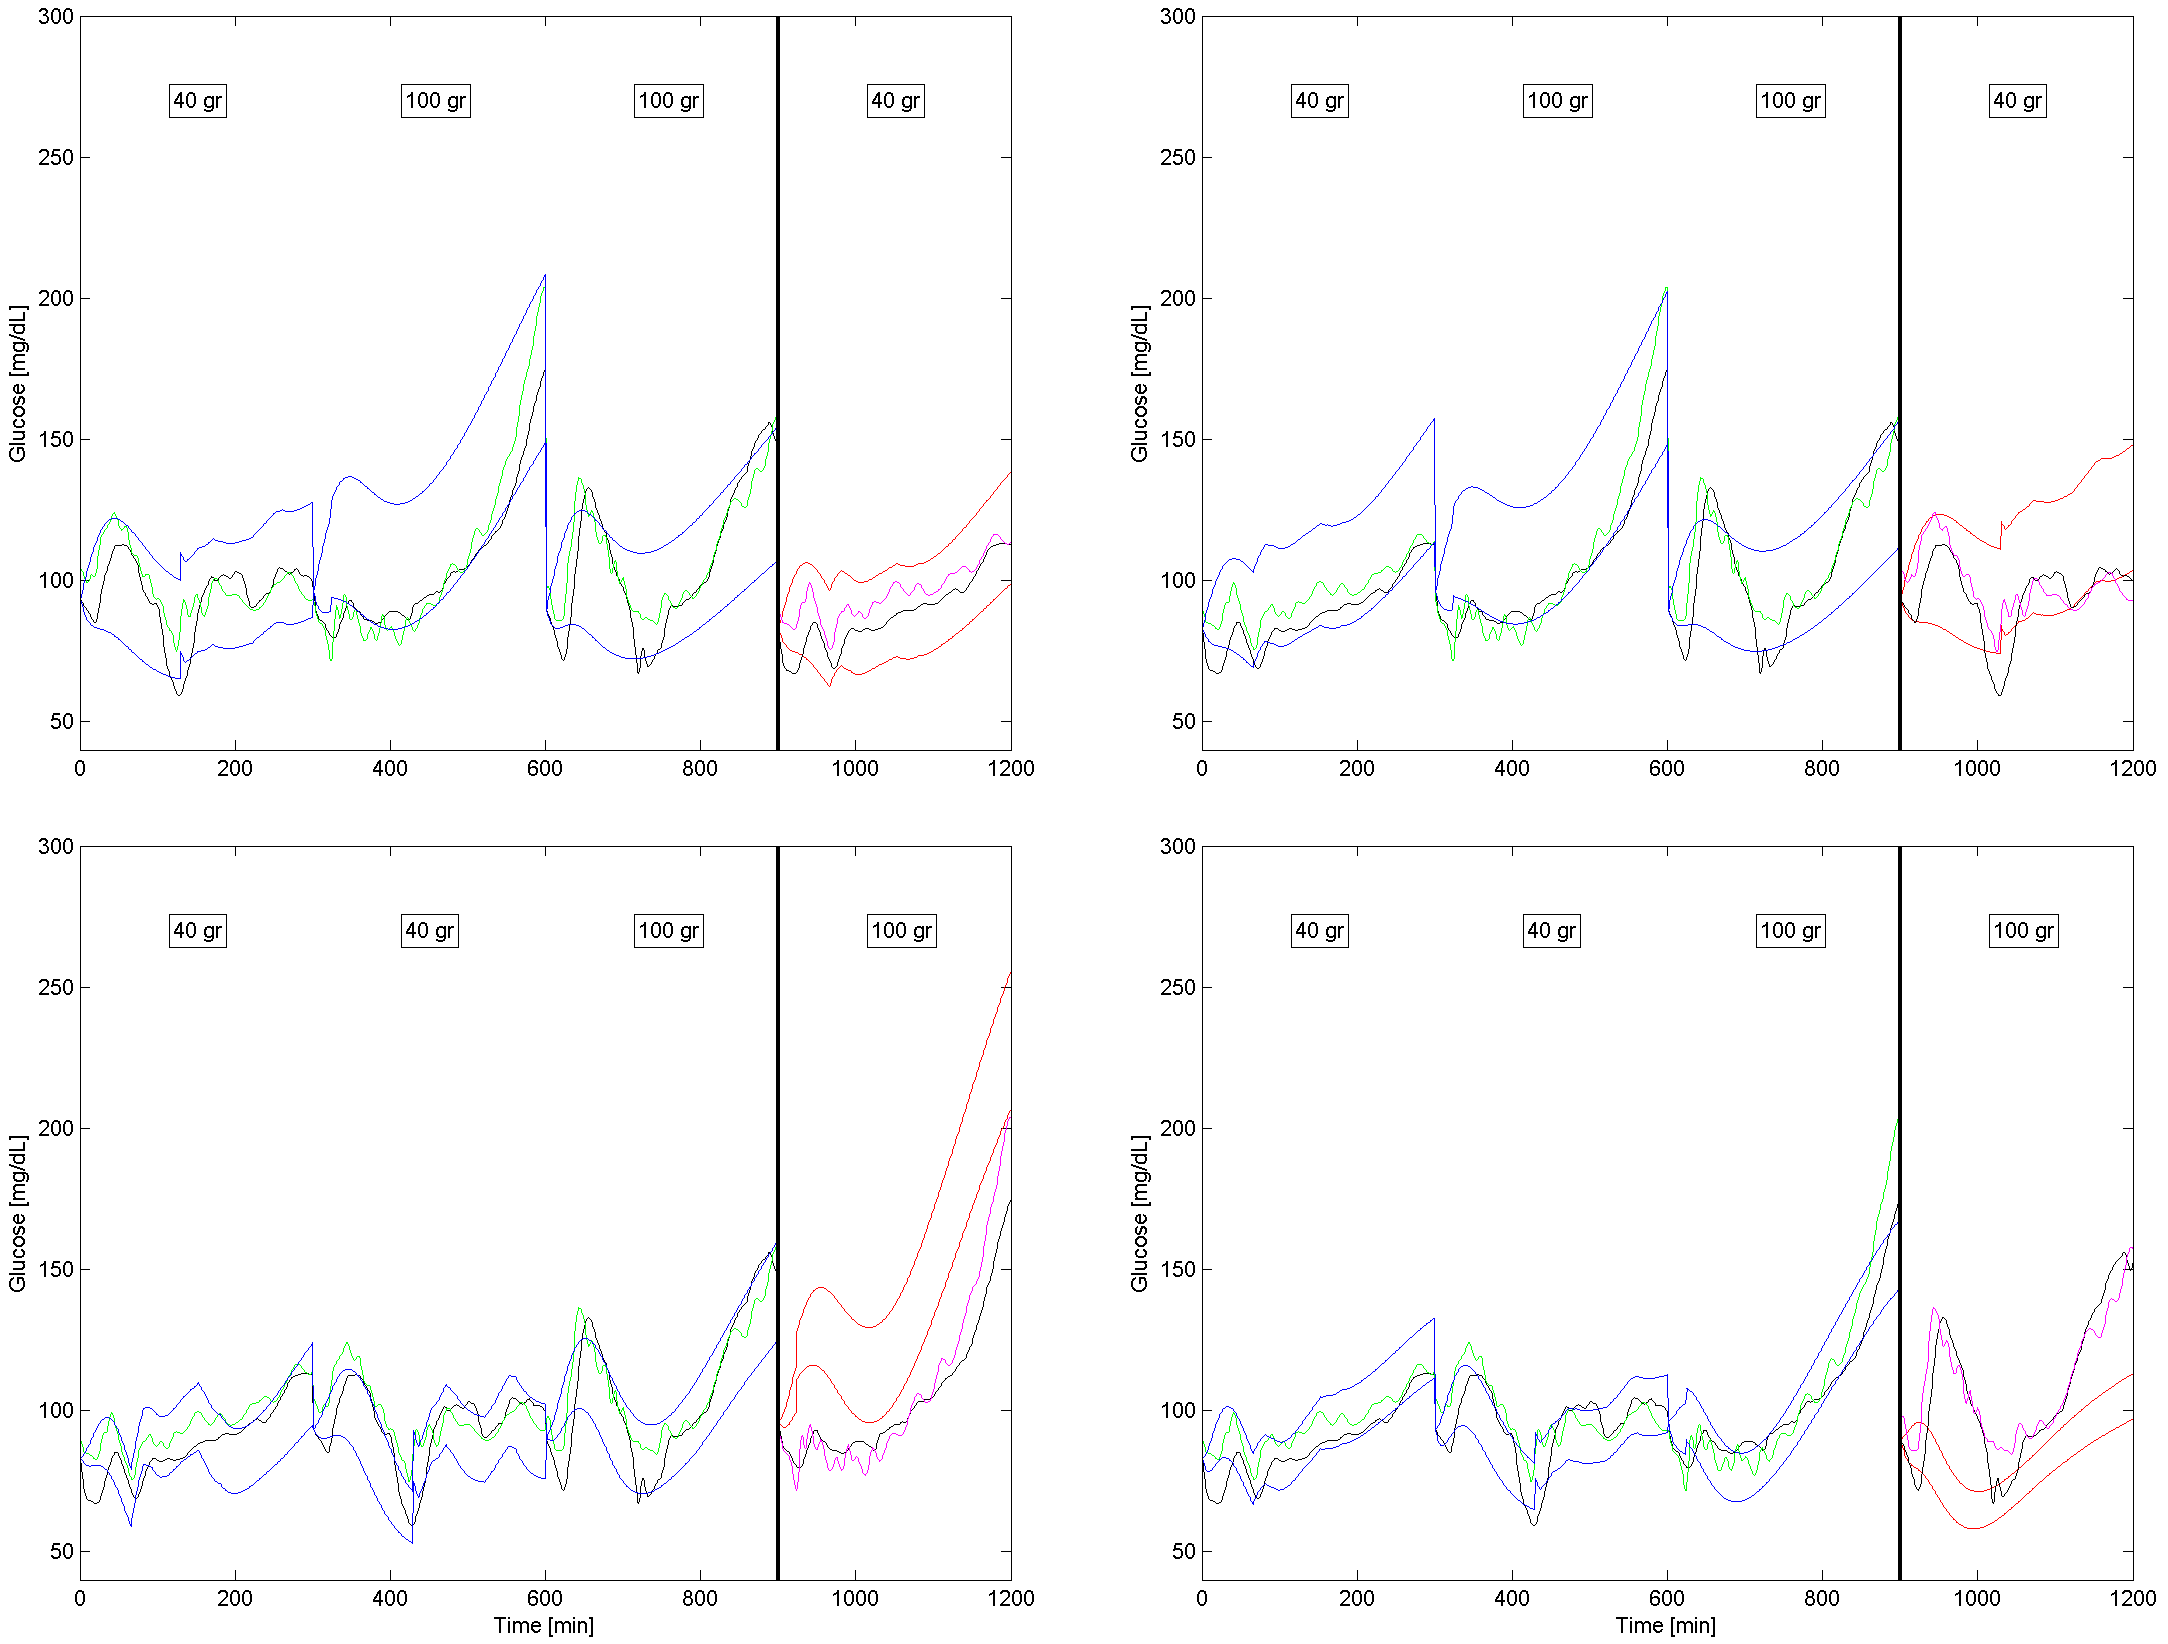
\epsfig{file=Figures/CGM_patient_6.png, width=\textwidth}\caption{Patient 6 identification and validation results for the scenario C100. Day 1 validation is shown top left. Top Right graph shows validation for day 2. Bottom left validates day 3. Bottom right shows validation for day 4. Black lines represent the CGM signal. YSI measurements are displayed in green for the identification days, and in magenta for the validation day.}
\label{fig:CGMpatient6}.
\end{figure}

Patient 6 can be categorized as a patient with very low variability. Envelope widths are much lower that with the rest of the patients. Also, glucose excursions for this patient are smaller than the rest of the dataset. This permits a clearer observation of the best case scenario of the patient. CGM readings are satisfactory for all the postprandial periods of this patient, resulting in good identification for the CGM identification too. The first permutation is the best example of satisfactory identification, where all the prediction band encloses the YSI measurements, even though the initial point of the model simulation is taken from the CGM signal (it is the only known data to the model). Permutation 2 is a very similar case of very good prediction, but in this case it is improved by the larger envelope widths caused by CGM identification, because this particular permutation of this patient did not perform as well with YSI identification due to the small width (therefore small variability) of the patient's identification days. The two last permutations' validation days are a clear example of both patient's extremes of variability within the 4-day experiment, falling both of them out of the prediction bands

Patient's 6 example hints that the best case permutation hypothesis that was proved valid in the previous chapters is still possible for the CGM identifications. Best case validation metrics and envelope fitness measure are listed in table \ref{tab:resultsCGMbestcase}.

\begin{table}[hbtp]
	\centering
	\begin{tabular}{| c | c | c | c | c | c | c | c |} 
	\hline
	\multicolumn{2}{|c|}{$\gamma$} & 100 & 85 & 70 & 55 & 40 & 25 \\											
	\hline
	env\_fit & mean & 27.3 & 26.8 & 25.8 & 25.4 & 24.9 & 22.5 \\
	(mg/dL) & median & 22.1 & 21.8 & 20 & 19.4 & 20 & 16 \\
	\hline
	Width & mean & 130.4 & 127 & 122.5 & 112 & 112.3 & 91 \\
	(mg/dL) & median & 115.4 & 110.8 & 113.1 & 102.9 & 95.1 & 67.6 \\
	\hline
	Prediction & mean & 90.9 & 90.6 & 88.3 & 82.1 & 89.9 & 80.1 \\
	(\%) & median & 97.8 & 97.3 & 96.7 & 97.2 & 97 & 96.2 \\
	\hline
	MARD & mean & 0.58 & 0.59 & 0.74 & 1.82 & 0.81 & 2.06 \\
	(\%) & median & 0.14 & 0.15 & 0.19 & 0.19 & 0.2 & 0.27 \\
	\hline
	gMARD & mean & 0.59 & 0.6 & 0.75 & 1.83 & 1.02 & 3.15 \\
	(\%) & median & 0.14 & 0.15 & 0.19 & 0.19 & 0.2 & 0.27 \\
	\hline
\end{tabular}
\caption{Results for all the $\gamma$ values for the best case permutation in each patient. \textit{env\_fit} values correspond to identification days, and the rest of metrics to the validation days}
\label{tab:resultsCGMbestcase}
\end{table}

MARD measures are very small, comparable in magnitude with those of the previous chapters. gMARD difference form the MARD counterpart is no relevant and supposes no danger to the patients. Average predicted samples is approximately 90\% for all $\gamma$ values considered, therefore consideration of full coverage of the validation days for the best case identification is valid.

When comparing the metrics of the best cases with the whole dataset, even though widths appear to be larger for the best cases (122,5 mg/dL > 95,95 mg/dL) this difference is actually no significant(p=0.109) because of the small number of best case samples available. It was discussed before in this section how the small number of patients is one of the main problems for the validation of the methodology at stake in this thesis. This problem gets aggravated by the removal of the two patients whose CGM was faulty, effectively reducing the samples size 16\%. Significant differences in the metrics are much more difficult to find in smaller samples of the diabetic patient's population. Nevertheless, envelope fitness of the best cases at stake was not different from that of the whole dataset (21.75 mg/dL > 21.49 mg/dL; p=0.457), validating the fitting process.

\section{Discussion}
\label{sec:CGMdiscussion}

Full model patient identification considering uncertainty has been performed in this chapter, from both YSI and CGM data sources, displaying the decreasing prediction capabilities of the models involved as the complexity of the system is increased and the data source loses quality (the associated error increases).

For the identification including the subcutaneous insulin route, 8 different scenarios were tested for identification feasibility composing different parameter vector to be used in the identification. Even though all the parameters in the model were identifiable following the theoretical identifiability tests performed, each parameter was left out of the identification sequentially in order to test the practical identifiability of the others, along with the prediction capabilities of the model with each combination of parameters. Only parameter $\beta$, corresponding to the aggregated error parameter of the subcutaneous insulin route, was discarded due to identifiability problems.

The inclusion of CGM supposed a great set-back for the prediction power of the models identified. The width associated for the selected optimum scenario was in average 95.9 mg/dL (median 85.6 mg/dL), far away of the average 82.4 mg/dL (median 72.7 mg/dL) necessary for the YSI study that included the subcutaneous route of insulin. When these figures are compared to the 78.8 mg/dL (median 66.4 mg/dL) width obtained in the in-patient study, it is possible to view the error introduced by the CGM devices (difference of 13.5 mg/dL) in comparison to the model mismatch introduced by the subcutaneous insulin route of 3.6 mg/dL.

Prediction error increased with the inclusion of the subcutaneous route and the CGM measurements. Starting with a MARD of 7.61\% (median 5.56\%) in the in-patient study, this error metric increased up to 9.63\% (median 4.34\%) with the subcutaneous insulin route inclusion in the model, and even larger error was reported for with the inclusion of continuous monitoring technology, up to 10.04\% (median 5.14\%). When comparing the increment of envelope width and MARD, it can be appreciated that most of the uncertainty from the CGM inclusion is translated into envelope width by the prediction algorithm, while the inclusion of the input model for subcutaneous insulin contributes to the methodology by increasing the MARD. This is a consequence of the choice of a $\gamma=100$ for both experiments involving YSI data, weighting the envelope width similarly in the optimizations for both experiments. $\gamma$ value was smaller for the CGM experiment, giving more importance to error minimization and therefore increasing the envelope width.

Best case permutations are identified for both YSI identifications and CGM identifications. The inclusion of more complex models (subcutaneous insulin route) or inaccurate measurements (CGM) does not affect the outcome of the maximum variability identification, which always presents a very good solution to each patient. Best case validation bands cover almost all the validation data, reinforcing the utility of the method for variability predictions.

Finally, the number of patients is the great limitation to the findings here exposed. CGM errors and model mismatches suppose a great challenge to the identification techniques available, introducing relevant misestimation in the final performance metrics used for evaluation of the identification methodologies, which will only be palliated if large databases of patients' information are available to the scientific community.






